%%%%%%%%%%%%%%%%%%%%%%%%%%%%%%%%%%%%%%%%%%%%%%%%%%%%%%%%%%%
% --------------------------------------------------------
% Tau
% LaTeX Template
% Version 2.4.4 (2/06/2026)
%
% Author:
% Omar Ayman Tawfiq Bakr (bakro0298@gmail.com)
%
% License:
% Creative Commons CC BY 4.0
% --------------------------------------------------------
%%%%%%%%%%%%%%%%%%%%%%%%%%%%%%%%%%%%%%%%%%%%%%%%%%%%%%%%%%%

\documentclass[9pt,a4paper,twocolumn,twoside]{tau-class/tau}
\usepackage[english]{babel}
\usepackage{enumitem}
\usepackage{hyperref}
\usepackage{fontawesome5}

%----------------------------------------------------------
% TITLE
%----------------------------------------------------------

\journalname{Summary Report }
\title{Volleyball-Group-Activity-Recognition}

%----------------------------------------------------------
% AUTHORS, AFFILIATIONS AND PROFESSOR
%----------------------------------------------------------

\author[a,1]{Omar Ayman Tawfiq Bakr \href{bakro0298@gmail.com}{\faGoogle}
 \href{https://www.linkedin.com/in/omarrbakr/}{\faLinkedinIn } \href{https://github.com/omarTBakr}{\faGithub} }

%----------------------------------------------------------
% FOOTER INFORMATION
%----------------------------------------------------------

\footinfo{Summary Report}
\theday{July 14, 2026}
\leadauthor{Omar Ayman Bakr}
\course{Volleyball-Group-Activity-Recognition}

%----------------------------------------------------------
% ABSTRACT AND KEYWORDS
%----------------------------------------------------------

\begin{abstract}
   A condensed summary of the Volleyball Group Activity Recognition project: the data pipeline, the generic multi-baseline loader, and the four completed baselines --- B1, a single-frame fine-tuned ResNet-50 (62.6\% test accuracy / 0.630 macro F1); B3, a person-then-group crop classifier (60.7\% / 0.589); B4, a temporal classifier that runs an LSTM over B1's frozen frame features (66.1\% / 0.673, best macro F1); and B5, a per-player temporal model that pools LSTM summaries of each player's crop sequence (66.3\% / 0.619, best accuracy). The dataset (Ibrahim et al., CVPR 2016) contains 55 videos / 4{,}830 clips with 8 scene-level group activities and 9 player-level actions.
\end{abstract}

%----------------------------------------------------------

\keywords{\ Volleyball, Group Activity Recognition, CNN, RNN, LSTM, ResNet50, Classification, Multiclass Classification, Transfer Learning}

%----------------------------------------------------------

\begin{document}

    \maketitle
    \thispagestyle{firststyle}
    \tauabstract

%----------------------------------------------------------

\section{Problem \& Dataset}

    \taustart{V}olleyball Group Activity Recognition is a hierarchical classification problem: predict the scene-level group activity (8 classes: \texttt{l/r}-pass, -spike, -set, -winpoint) and the per-player action (9 classes: blocking, digging, falling, jumping, moving, setting, spiking, standing, waiting). The dataset comes from \href{https://www.cs.sfu.ca/~mori/research/papers/ibrahim-cvpr16.pdf}{``A Hierarchical Deep Temporal Model for Group Activity Recognition''} (Ibrahim et al., CVPR 2016; \href{https://github.com/mostafa-saad/deep-activity-rec}{official repo}, \href{https://www.kaggle.com/datasets/ahmedmohamed365/volleyball}{Kaggle mirror}).

Key facts: \textbf{55 videos, 4{,}830 clips} (train/val/test = 2{,}152/1{,}341/1{,}337 clips over disjoint video splits of 24/15/16). Each clip has \textbf{41 frames}; the clip folder is named after its annotated \emph{middle frame}. Both label levels are heavily skewed: \texttt{standing} is $\approx$68\% of person actions, and \texttt{l/r\_winpoint} are $\approx$2.5$\times$ rarer than the other group classes. The group classes come in \textbf{left/right mirror pairs}, so horizontal geometry is part of the label --- the transform pipelines therefore use no horizontal flips and warp inputs directly to $224 \times 224$ so the full court (or the full player) always stays in view.

\section{Data Pipeline}

Three raw annotation sources (action detections, person detections, player tracking) are unified by a two-stage parser (\texttt{src/json\_parser.py}) into one master JSON keyed \texttt{video\_id/clip\_id}, then enriched with the group-activity label per clip (looked up per video against each clip's own middle frame) and cached as a pickle ($\sim$247\,MB) for instant metadata loading. Frames are served either from a memory-mapped LMDB (local) or straight from disk (Kaggle); both backends expose the identical \texttt{VolleyballDataset}, which covers every baseline through flags: full frames or per-player crops, 1 or 9 frames per clip. A custom collate pads the variable player count per clip and returns a validity mask so padded slots never reach the loss or the pooling.

\section{Baseline Roadmap}

Table~\ref{tab:baselines} lists the planned progression of models, each adding temporal and/or player-level structure on top of the previous one.

\begin{table}[h]
    \centering
    \caption{Baseline models. All eight ladder models complete with results; B8 (team-split pooling) leads at 85.6\% test accuracy. B9 is the control: the same task with none of the player-level structure.}
    \label{tab:baselines}
    \begin{tabular}{lccc}
        \toprule
        \textbf{Model} & \textbf{Temporal} & \textbf{Player} & \textbf{Scene} \\
        \midrule
        B1 & --- & --- & Image clf. \\
        B3 & --- & Crop clf. & Concat-pool + MLP \\
        B4 & LSTM & --- & LSTM \\
        B5 & LSTM/player & Concat-pool & MLP \\
        B6 & LSTM/image & Max-pool/frame & LSTM + skip Conv1d \\
        B7 & LSTM$_1$ + LSTM$_2$ & Pool/frame & LSTM$_2$ + skips \\
        B8 & LSTM$_1$ + LSTM$_2$ & Team-split & LSTM$_2$ + skips \\
        \midrule
        B9 & --- & --- & YOLO frame clf. \\
        \bottomrule
    \end{tabular}
\end{table}

\section{Baseline 1: Single-Frame Classifier}

Fine-tunes a pretrained ResNet-50 on the clip's middle frame for the 8 group classes. Two-stage schedule: linear probe (head only, 10 epochs, lr $10^{-3}$), then partial fine-tune of \texttt{layer3/4} + head (up to 100 epochs, backbone lr $2.5 \times 10^{-4}$, head $3\times$, cosine annealing, batch 16, frozen BatchNorm held in eval).

\begin{table}[h]
    \centering
    \caption{Baseline 1 test-set metrics.}
    \label{tab:b1-metrics}
    \begin{tabular}{lc}
        \toprule
        \textbf{Metric} & \textbf{Value} \\
        \midrule
        Accuracy   & 62.60\% \\
        Macro F1   & 0.630 \\
        Test Loss  & 1.42 \\
        \bottomrule
    \end{tabular}
\end{table}

Fig.~\ref{fig:b1-confusion} shows the per-class confusion on the test split.

\begin{figure}[h]
    \centering
    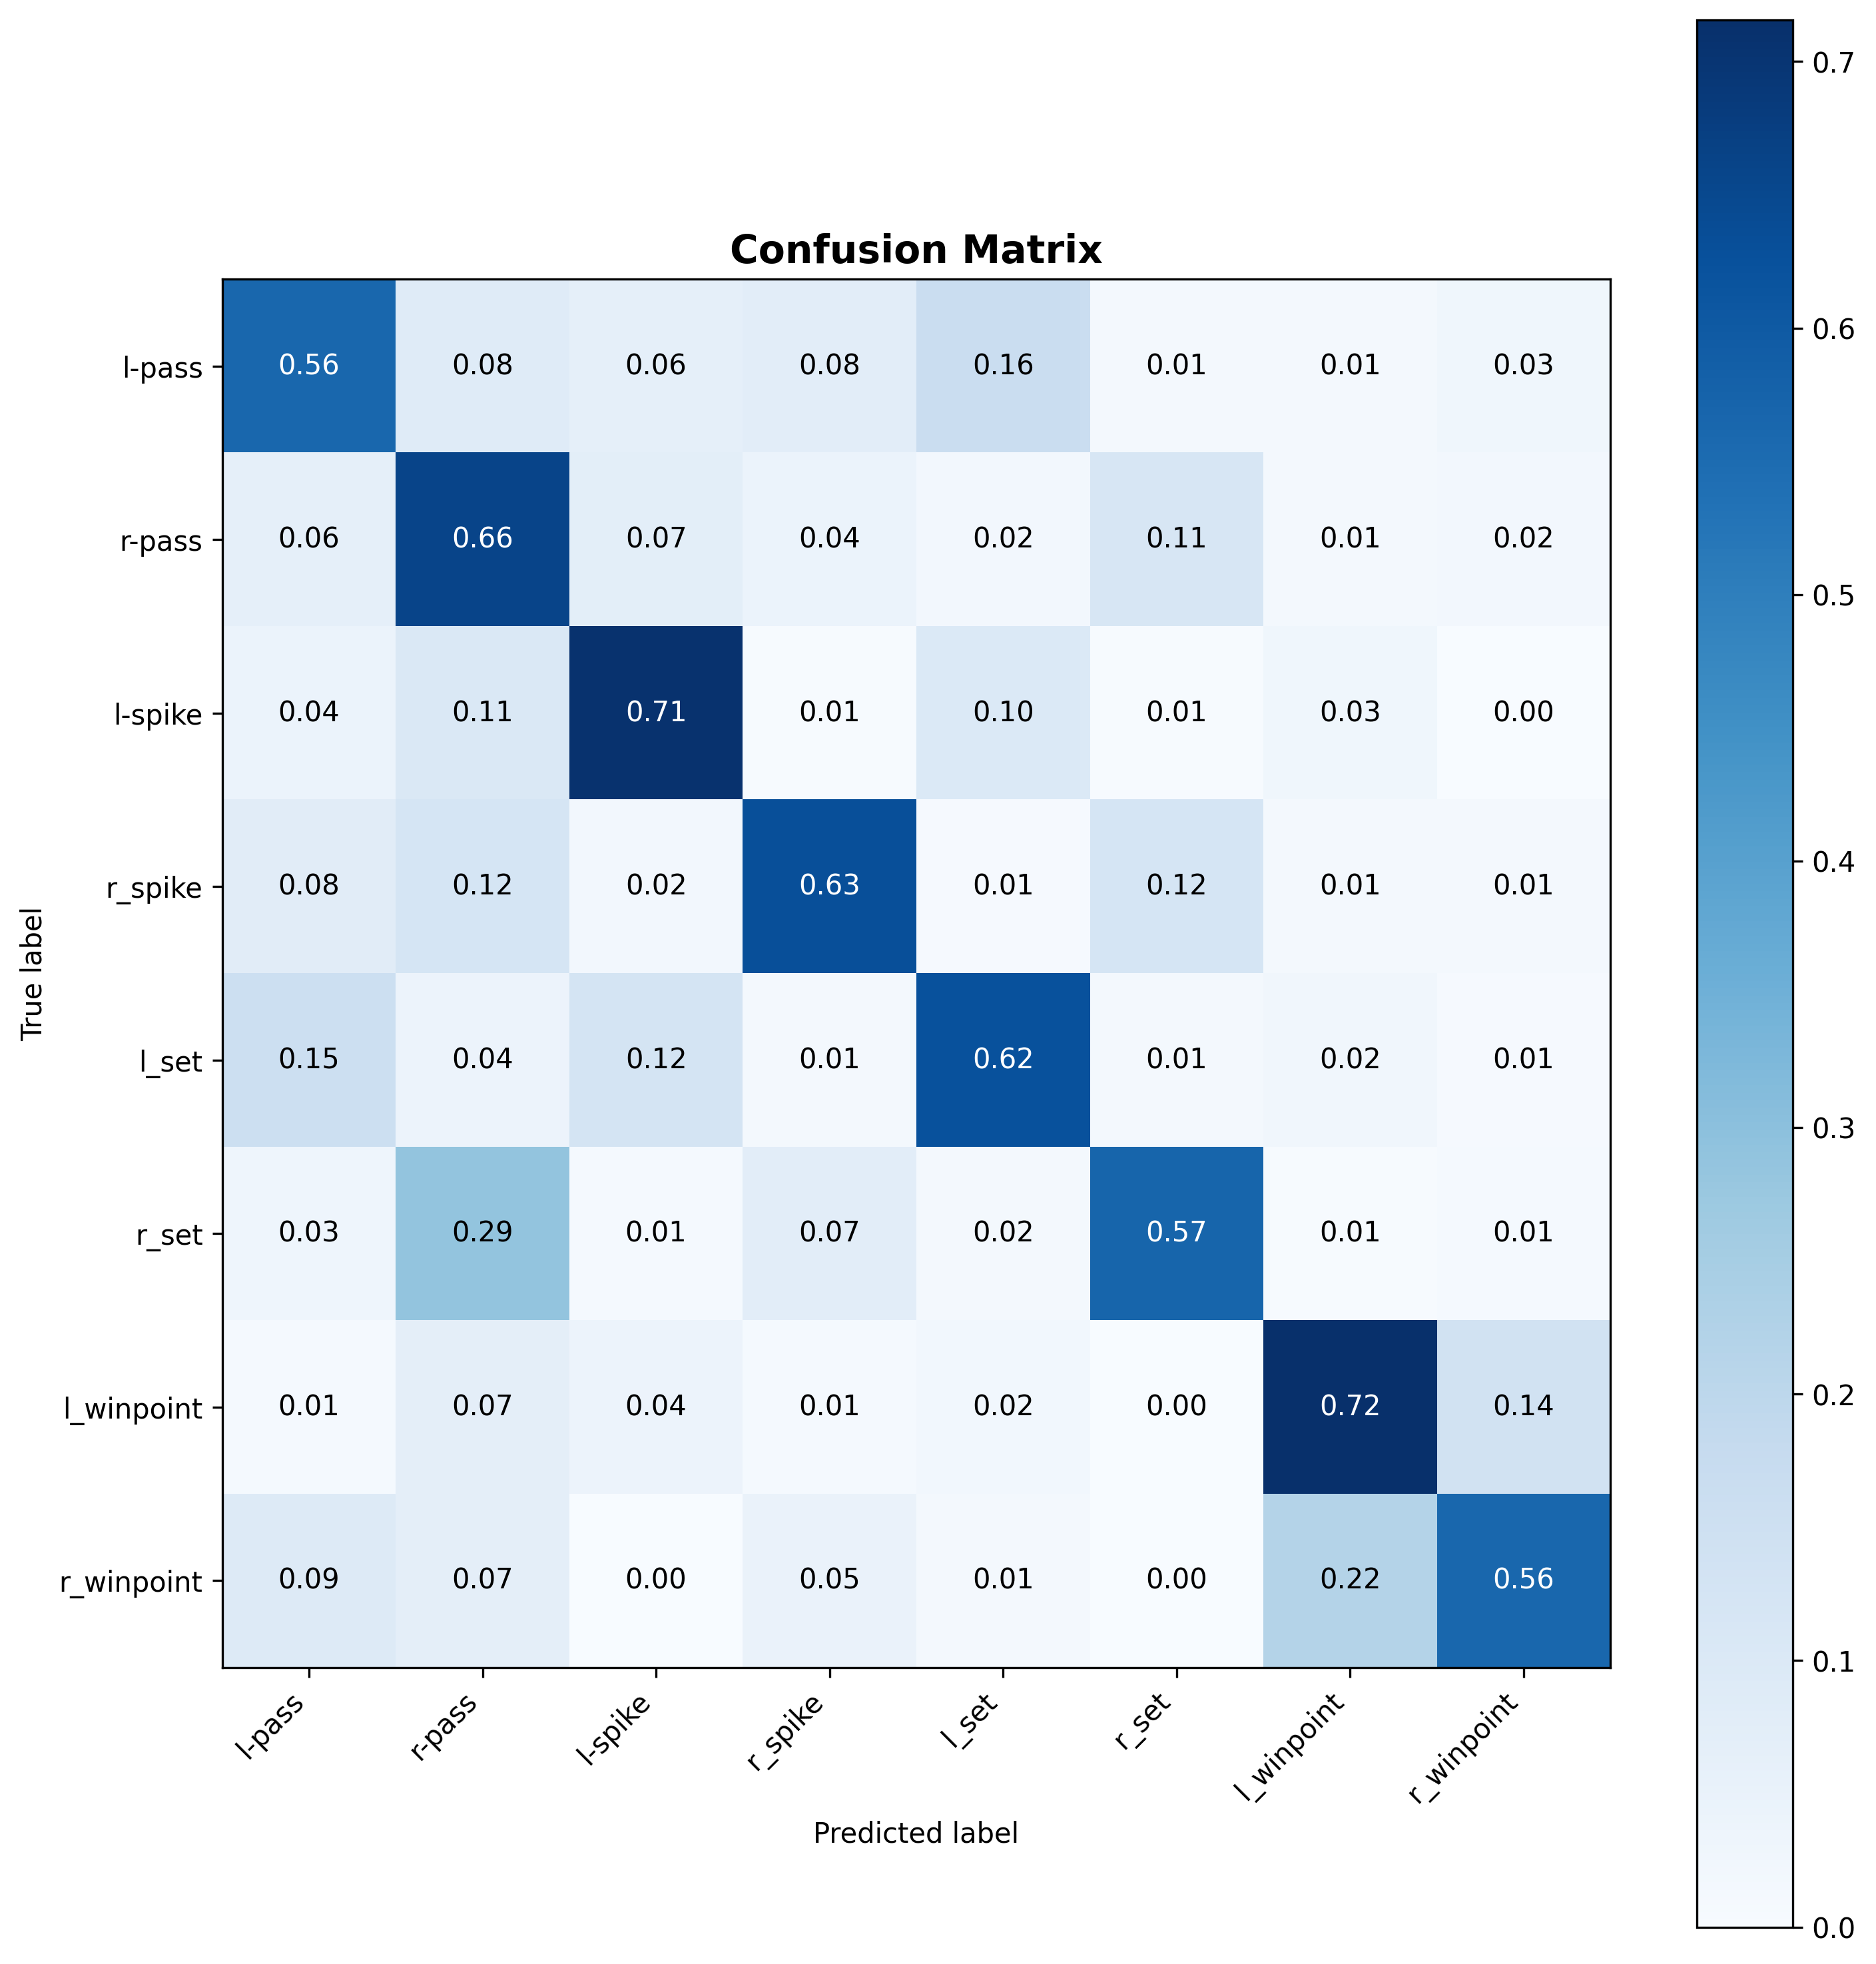
\includegraphics[width=0.95\linewidth]{figures/b1_confusion_matrix.png}
    \caption{Baseline 1 test confusion matrix.}
    \label{fig:b1-confusion}
\end{figure}

\section{Baseline 3: Person-Then-Group}

\textbf{Stage A} fine-tunes ResNet-50 on individual player crops for the 9 person actions with inverse-frequency class-weighted CE (without it the loss collapses onto \texttt{standing}). \textbf{Stage B} freezes that backbone, extracts a $(P, 2048)$ feature matrix per clip, concatenates masked max- and mean-pooling across players ($2 \times 2048$), and trains an MLP ($4096 \to 512 \to 8$, Dropout 0.4) with class-weighted CE for the group classes. SGD (momentum 0.9, Nesterov), 50 epochs and patience 10 per stage, batch 16 clips, \texttt{nn.DataParallel} on multi-GPU hosts. Stage A reaches 70.4\% validation accuracy (macro F1 0.512) on the person actions; Stage B 60.0\% (0.584) on the group activities.

\begin{table}[h]
    \centering
    \caption{Baseline 3 test-set metrics.}
    \label{tab:b3-metrics}
    \begin{tabular}{lc}
        \toprule
        \textbf{Metric} & \textbf{Value} \\
        \midrule
        Accuracy   & 60.73\% \\
        Macro F1   & 0.589 \\
        Test Loss  & 1.09 \\
        \bottomrule
    \end{tabular}
\end{table}

Fig.~\ref{fig:b3-confusion} shows the dominant error mode: left/right mirror confusion within each activity pair, worst on the rare \texttt{r\_winpoint}. The main open issue is \textbf{overfitting} (train $\approx$95\% vs.\ val 58--70\%), to be addressed with stronger augmentation, higher dropout, and earlier stopping in a follow-up run.

\begin{figure}[h]
    \centering
    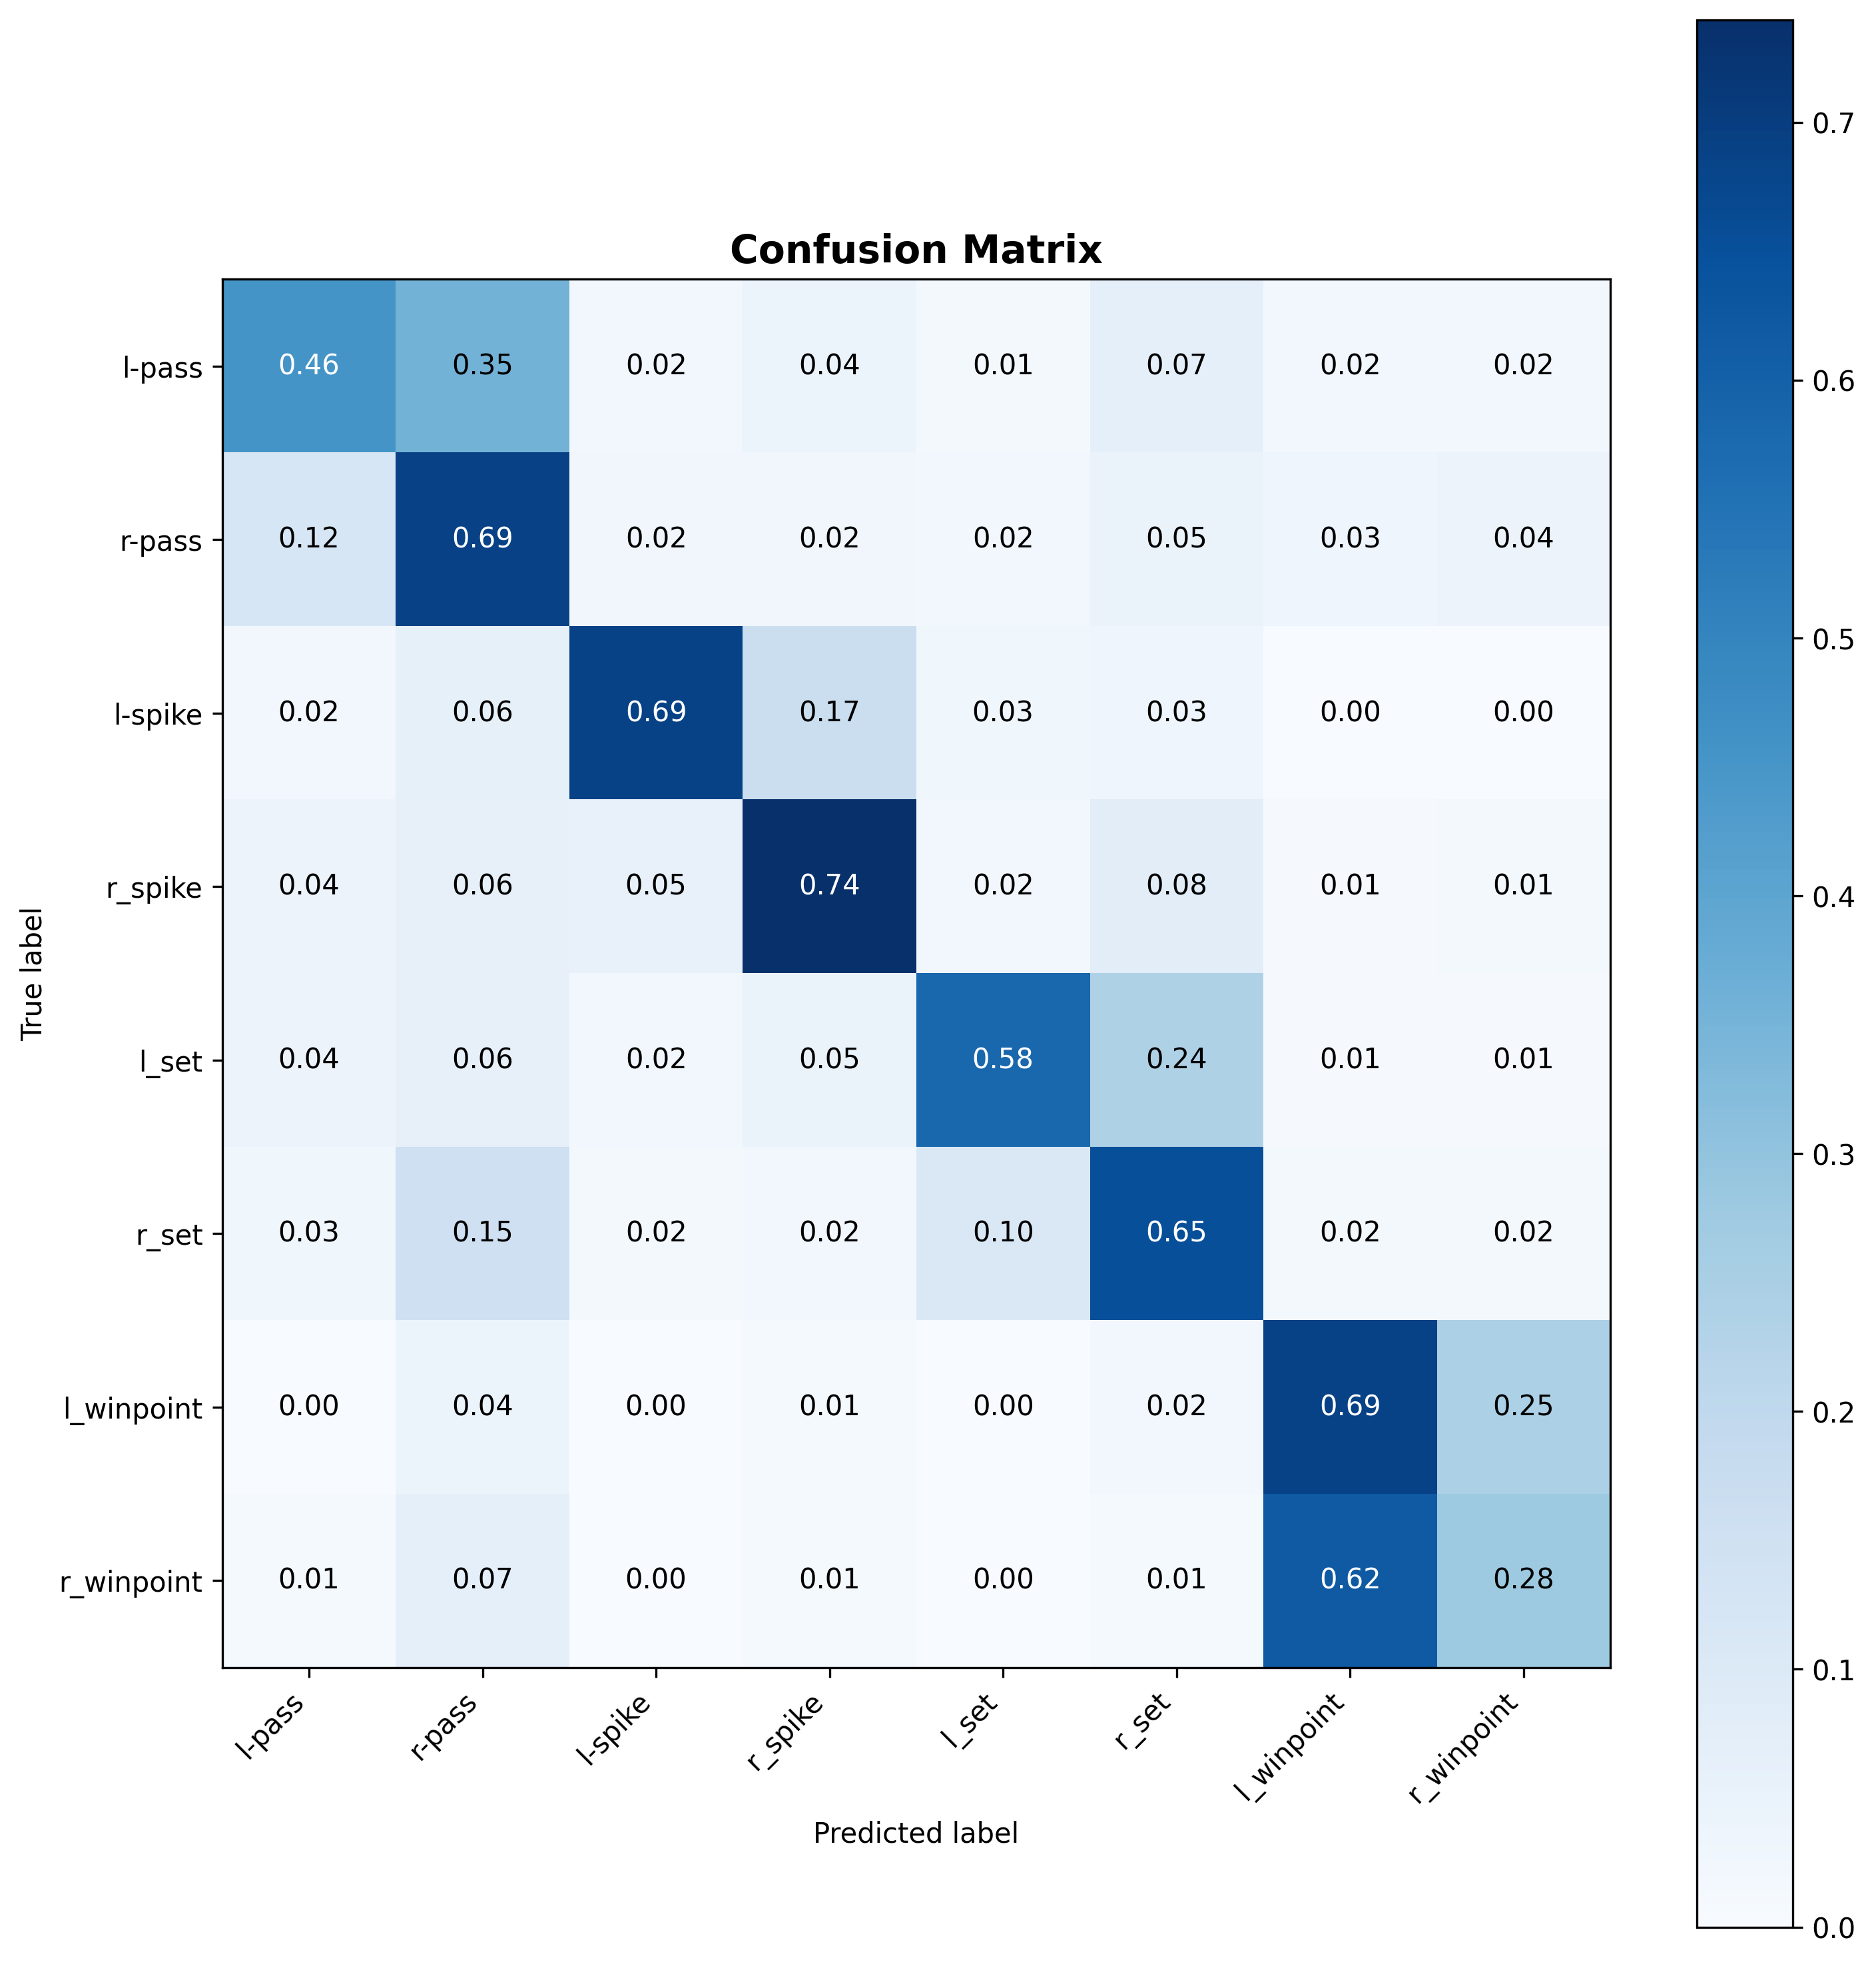
\includegraphics[width=0.95\linewidth]{figures/b3_confusion_matrix.png}
    \caption{Baseline 3 test confusion matrix.}
    \label{fig:b3-confusion}
\end{figure}

\section{Baseline 4: Temporal Image Classifier}

Each clip's 9-frame window is pushed through a \textbf{frozen} feature extractor loaded from Baseline 1's fine-tuned backbone, producing a $(9, 2048)$ feature sequence per clip. A single-layer LSTM (hidden 512) consumes the sequence and its final hidden state is classified by a small MLP head ($512 \to 256 \to 8$, Dropout 0.3). Only the LSTM + head train ($\approx$5.4M parameters; SGD lr $10^{-3}$, cosine annealing, class-weighted CE, batch 16 clips).

\begin{table}[h]
    \centering
    \caption{Baseline 4 test-set metrics.}
    \label{tab:b4-metrics}
    \begin{tabular}{lc}
        \toprule
        \textbf{Metric} & \textbf{Value} \\
        \midrule
        Accuracy   & \textbf{66.12\%} \\
        Macro F1   & \textbf{0.673} \\
        Test Loss  & 1.05 \\
        \bottomrule
    \end{tabular}
\end{table}

B4 is the strongest baseline so far: temporal context over B1's own features is worth \textbf{+3.5 accuracy points / +0.043 macro F1} versus B1's single-frame result --- the first direct evidence in this project that motion carries group-activity signal. Convergence is very fast (best validation F1 at epoch 4; training accuracy $\approx$99\% by epoch 14, where early stopping fired), repeating the overfitting pattern of B1/B3. Fig.~\ref{fig:b4-confusion} shows the test confusion matrix.

\begin{figure}[h]
    \centering
    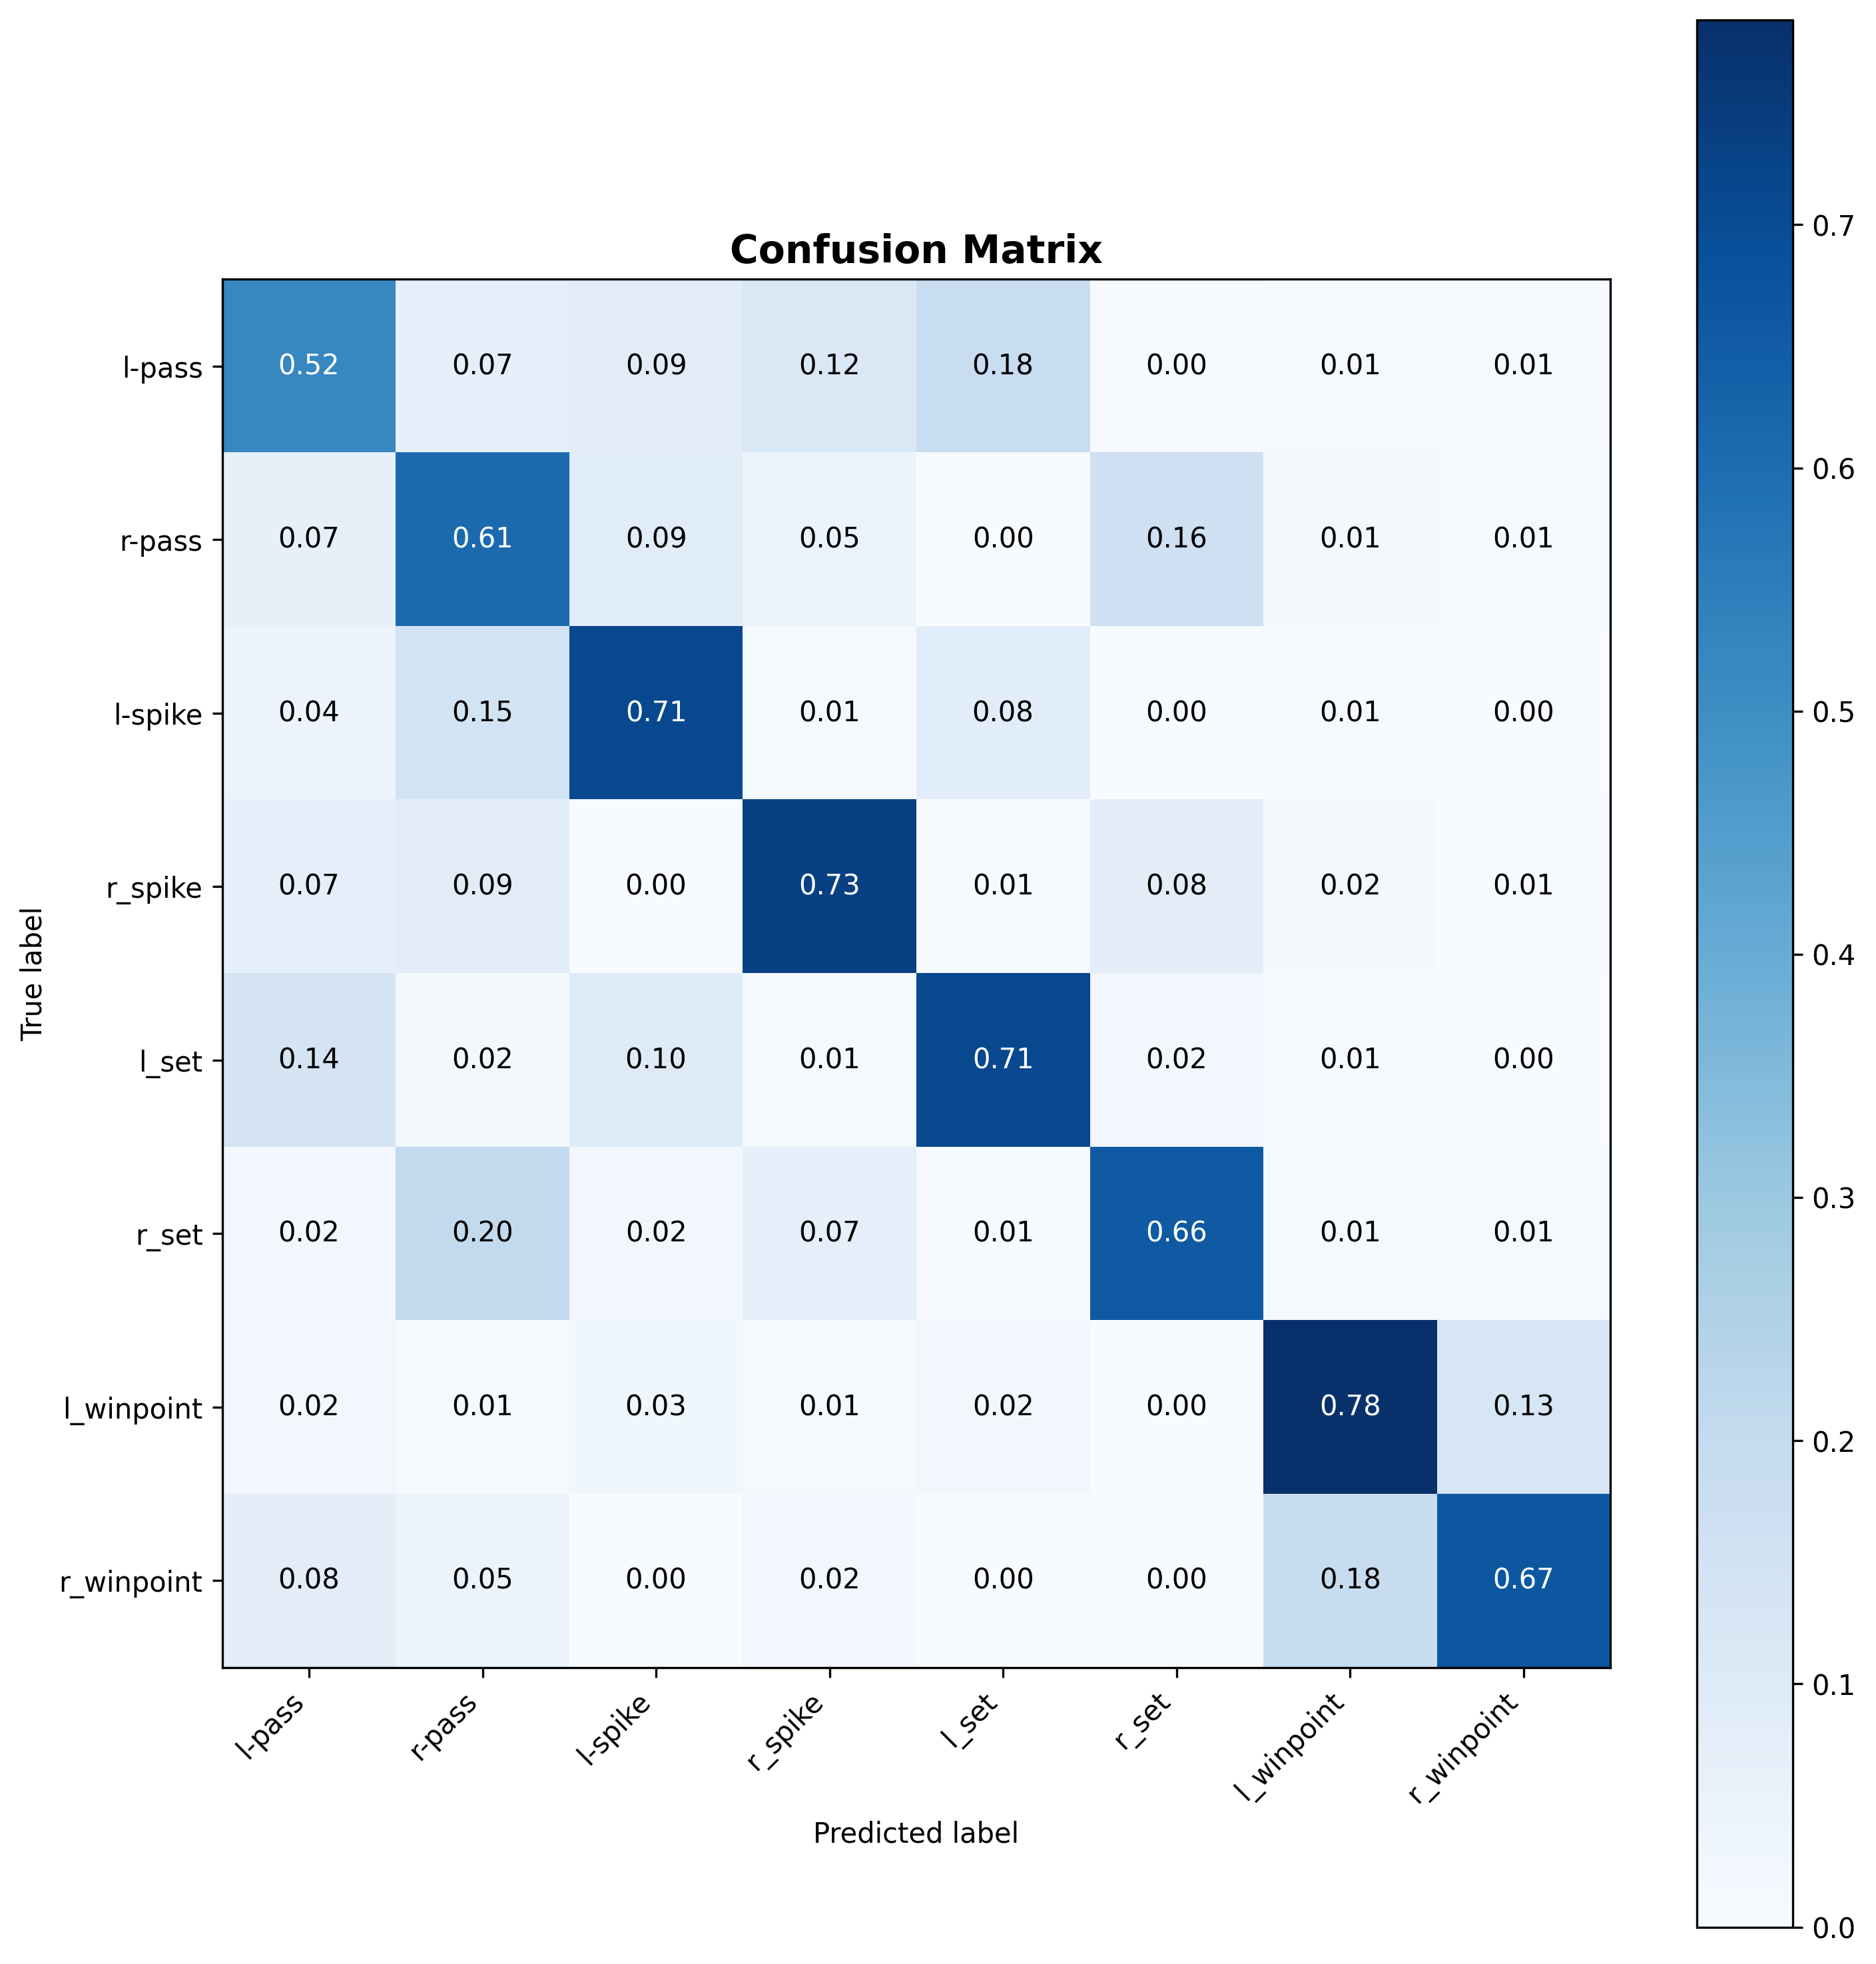
\includegraphics[width=0.95\linewidth]{figures/b4_confusion_matrix.png}
    \caption{Baseline 4 test confusion matrix.}
    \label{fig:b4-confusion}
\end{figure}

\section{Baseline 5: Temporal Person-Level Model}

A two-stage temporal extension of B3. \textbf{Stage A} feeds each player's 9-crop sequence through B3's \textbf{frozen} Stage-A person-action backbone and trains a shared LSTM (hidden 3072, 1 layer) + head to classify the 9 person actions from the sequence's final hidden state. \textbf{Stage B} freezes the Stage-A model entirely, computes one LSTM summary per player per clip, pools the summaries across players with masked concat (max $\|$ mean, classifier input $2 \times 3072$), and trains an MLP head ($6144 \to 3072 \to 1536 \to 8$, LayerNorm + Dropout 0.2) on the 8 group activities. Training uses SGD (lr $10^{-3}$, cosine annealing in Stage B), class-weighted CE in both stages, and gradient accumulation (effective batch 8 = micro 4 $\times$ 2) since each clip expands to $9 \times {\sim}12$ crop images.

\begin{table}[h]
    \centering
    \caption{Baseline 5 test-set metrics.}
    \label{tab:b5-metrics}
    \begin{tabular}{lc}
        \toprule
        \textbf{Metric} & \textbf{Value} \\
        \midrule
        Accuracy   & \textbf{66.34\%} \\
        Macro F1   & \textbf{0.619} \\
        Test Loss  & \textbf{0.97} \\
        \bottomrule
    \end{tabular}
\end{table}

B5 achieves the \textbf{best test accuracy and test loss of baselines B1--B5} (66.3\% / 0.97 vs.\ B4's 66.1\% / 1.05) and is markedly stronger on the core activities --- spike F1 reaches 0.78--0.80 and set 0.71 on both court sides, with cross-activity confusion nearly eliminated --- direct evidence that per-player temporal modeling adds signal beyond B4's scene-level features. Its macro F1 (0.619) nevertheless trails B4 (0.673) because of a single failure mode: \textbf{the \texttt{l/r\_winpoint} confusion is the worst left/right confusion of any baseline in this project}. As Fig.~\ref{fig:b5-confusion} shows, \texttt{r\_winpoint} collapses to 0.08 recall (F1 0.13), with 83\% of true \texttt{r\_winpoint} clips predicted as \texttt{l\_winpoint}. The cause is structural: orderless max/mean pooling over all ${\sim}12$ players erases which side of the net each player occupies; winpoint clips show both teams in near-identical celebration poses, so side identity is the only discriminative signal --- and the pooling destroys it. B8's team-split pooling (pool each team's six players separately, then concatenate) directly targets this failure.

\begin{figure}[h]
    \centering
    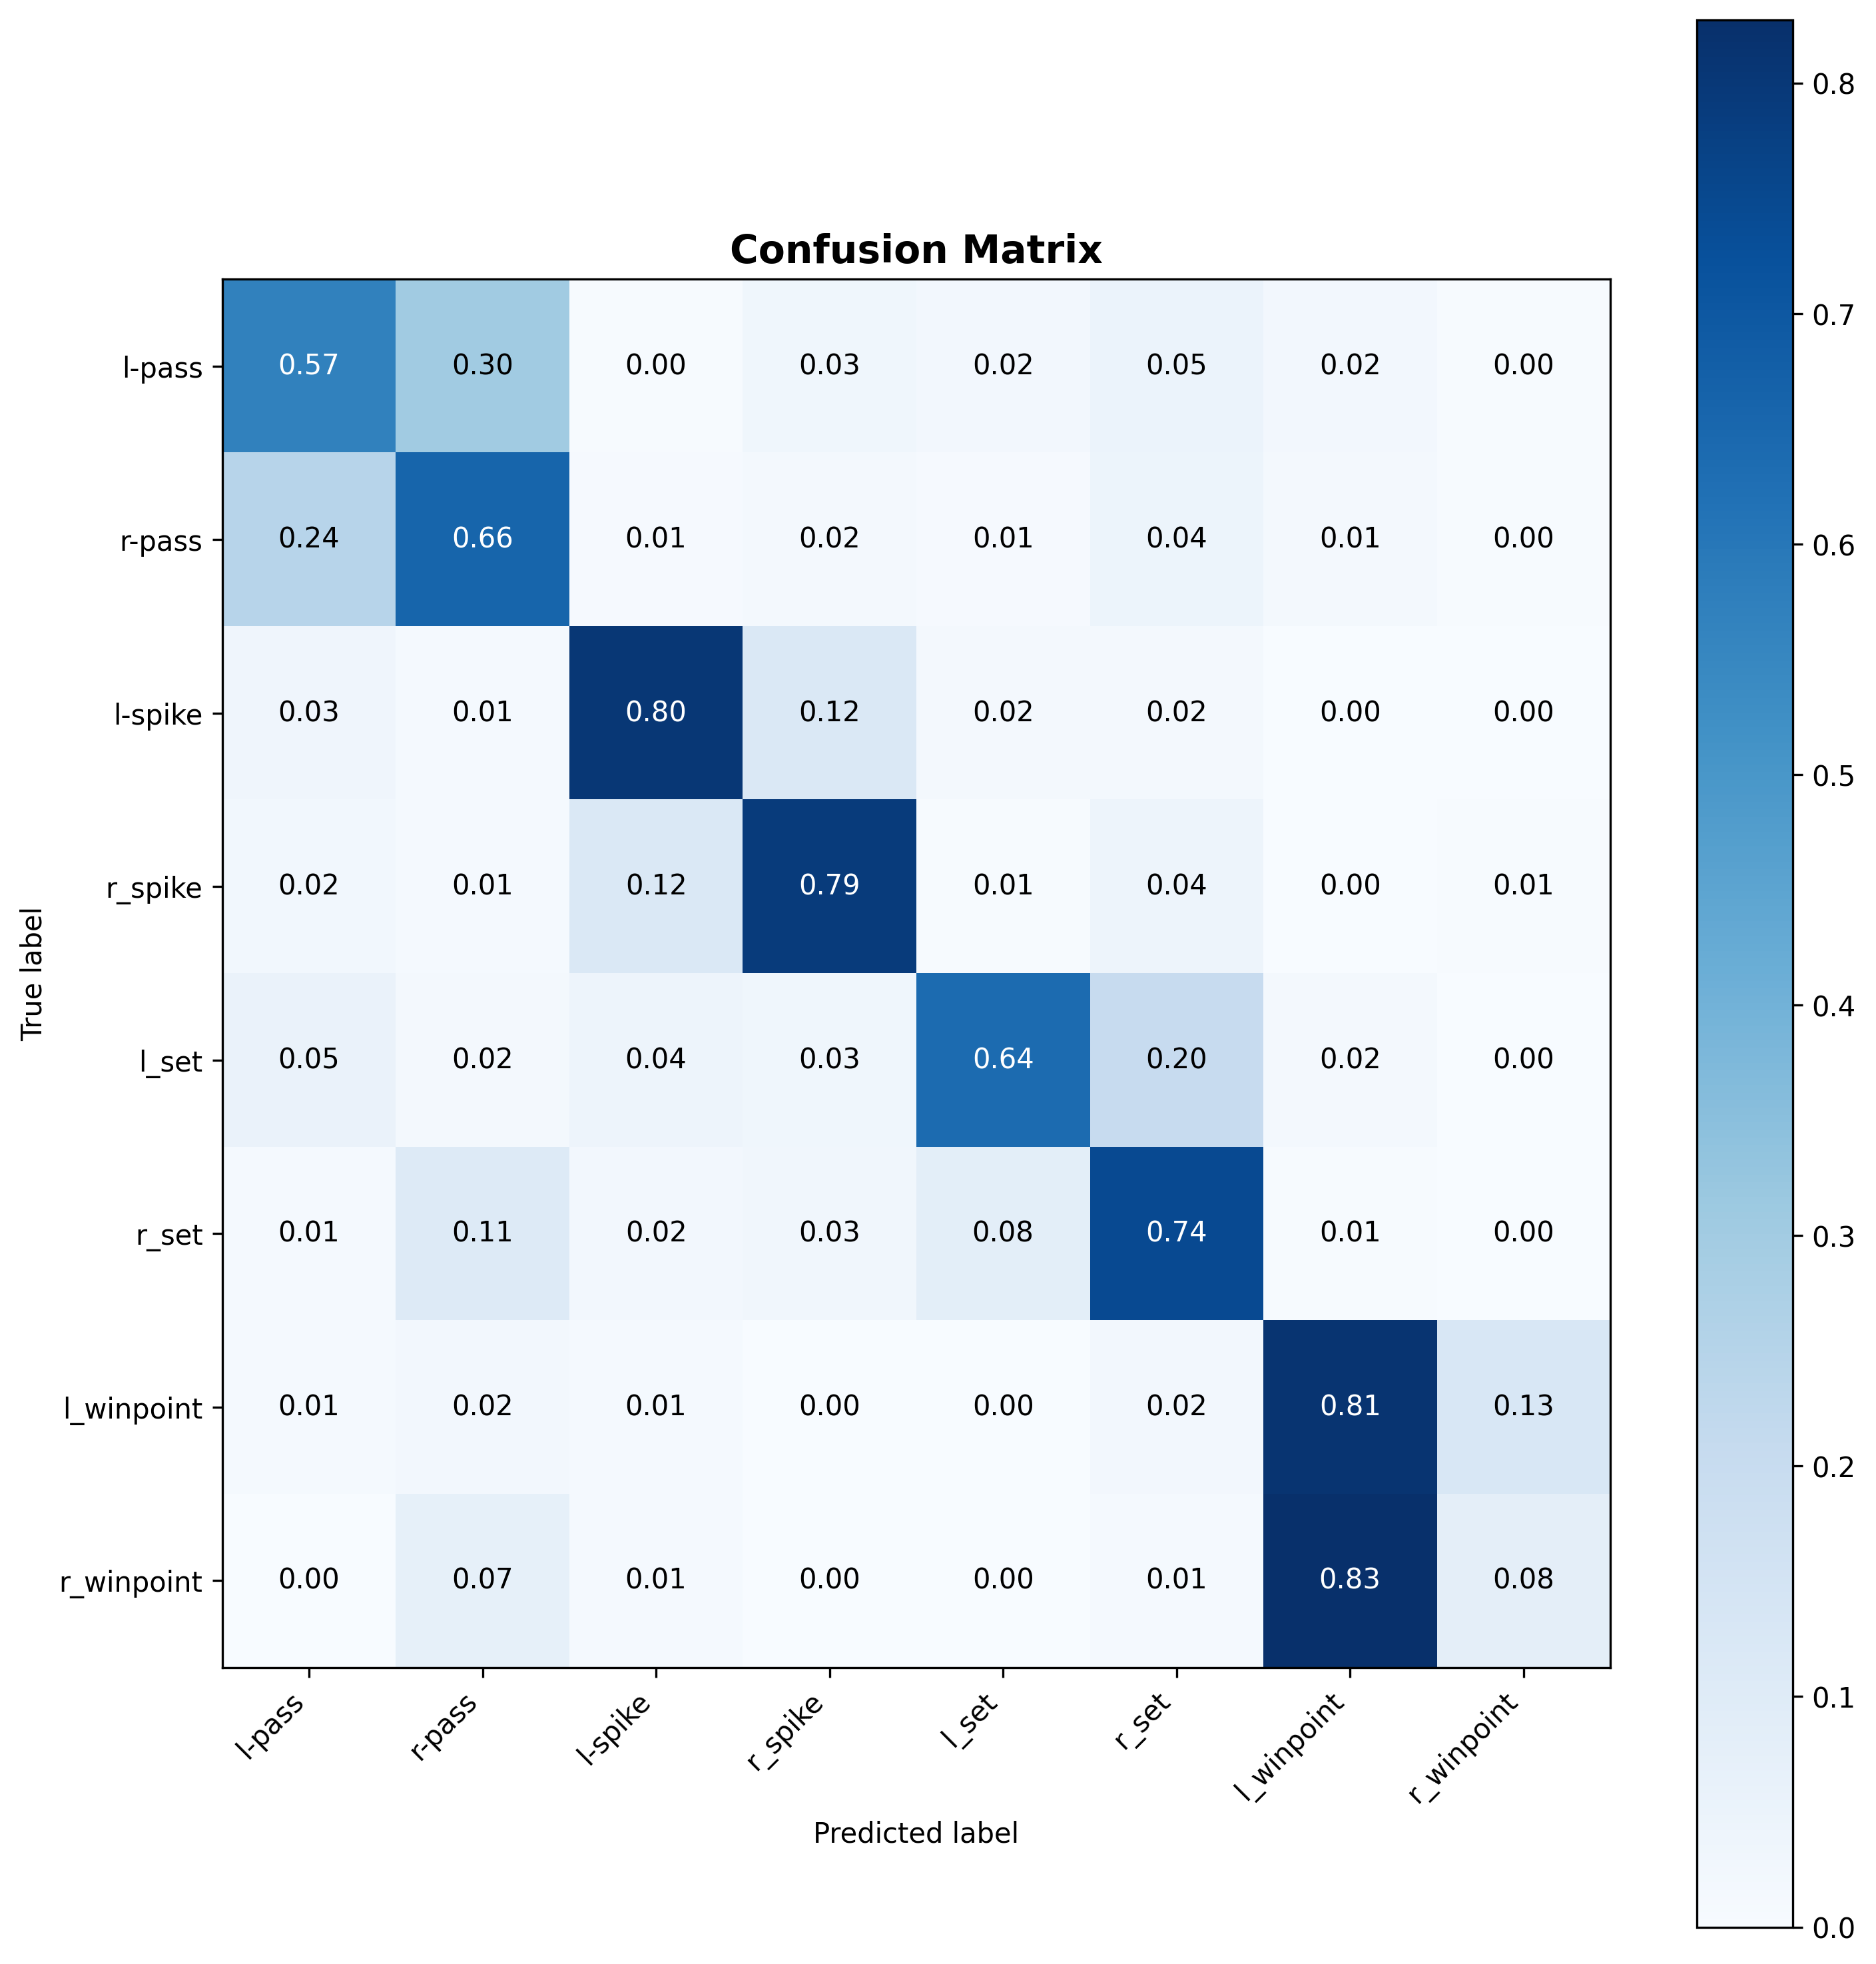
\includegraphics[width=0.95\linewidth]{figures/b5_confusion_matrix.png}
    \caption{Baseline 5 test confusion matrix. Note the \texttt{r\_winpoint} row: 83\% of its clips are predicted as \texttt{l\_winpoint} --- the side-blind pooling failure discussed in the text.}
    \label{fig:b5-confusion}
\end{figure}

\section{Baseline 6: Scene-Level Temporal Model}

B6 moves the temporal model from the player level (B5) to the \textbf{scene level}. Each frame's player crops pass through B3's \textbf{frozen} Stage-A backbone and are masked max-pooled across players \emph{per frame}, yielding a $(9, 2048)$ scene sequence per clip. An LSTM (hidden 512, 1 layer) consumes it; instead of keeping only the last hidden state, its 9 hidden states are concatenated \emph{along the time axis} with a linear projection of the pooled per-frame features (skip connection), giving $(18, 512)$, which a two-stage Conv1d with a global temporal kernel ($512 \to 256$, $k{=}18$, then $256 \to 128$, $k{=}1$) collapses into a 128-dim clip summary. \textbf{Stage A} pretrains LSTM + projection + Conv1d on the 9 person actions using single-player tracks ($P{=}1$, pooling is an identity). \textbf{Stage B} is two-phase: a 10-epoch \textbf{linear probe} (temporal model frozen, MLP head only, lr $10^{-3}$), then a \textbf{joint fine-tune} that unfreezes the temporal machinery with differential learning rates (temporal $10^{-4}$, head $10^{-3}$, cosine annealing, 50 epochs). The ResNet extractor stays frozen throughout; training otherwise matches B5 (class-weighted CE, label smoothing 0.01, effective batch 8 = micro 4 $\times$ 2).

\begin{table}[h]
    \centering
    \caption{Baseline 6 test-set metrics.}
    \label{tab:b6-metrics}
    \begin{tabular}{lc}
        \toprule
        \textbf{Metric} & \textbf{Value} \\
        \midrule
        Accuracy   & \textbf{70.53\%} \\
        Macro F1   & \textbf{0.686} \\
        Test Loss  & \textbf{1.04} \\
        \bottomrule
    \end{tabular}
\end{table}

B6 is the first baseline to lead on \emph{both} metrics: accuracy gains \textbf{+4.2 points over B5} (70.5\% vs.\ 66.3\%) and macro F1 passes B4's previous best (0.686 vs.\ 0.673). Scene-level temporal modeling over pooled person features corresponds to the paper's ``two-stage model without LSTM~1'' (74.7\% there); the remaining ${\sim}4$-point gap is consistent with our frozen rather than end-to-end backbone. The two-phase Stage B was decisive: the linear probe plateaued at 0.426 validation F1 --- a frozen LSTM pretrained only on person actions is a poor group-activity descriptor --- while joint fine-tuning lifted it to 0.646 ($+0.22$). The scene LSTM must see the group labels; the probe merely gives the head a stable start before the temporal weights move.

Per class (Fig.~\ref{fig:b6-confusion}), B6 is strongest on the acting-player activities (spike F1 0.86/0.82, set 0.72/0.69) and \textbf{halves B5's winpoint collapse without any team-aware pooling}: \texttt{r\_winpoint} recall recovers from 0.08 to 0.47 (F1 $0.13 \to 0.49$) and \texttt{l\_winpoint} reaches F1 0.55 --- scene-level temporal context evidently carries side information that per-player last-hidden summaries lost. Left/right confusion is nevertheless now the dominant remaining error: 47\% of true \texttt{r\_winpoint} is predicted \texttt{l\_winpoint}, l/r-pass leak 20--22\% into each other, and 21\% of \texttt{l\_set} is called \texttt{r\_set} --- the model is usually right about \emph{what} happened but guesses \emph{which side}. All-player max pooling remains side-blind; B8's team-split pooling targets exactly this. Overfitting persists (Stage A train F1 0.96 vs.\ val 0.54; fine-tune 0.93 vs.\ 0.64).

\begin{figure}[h]
    \centering
    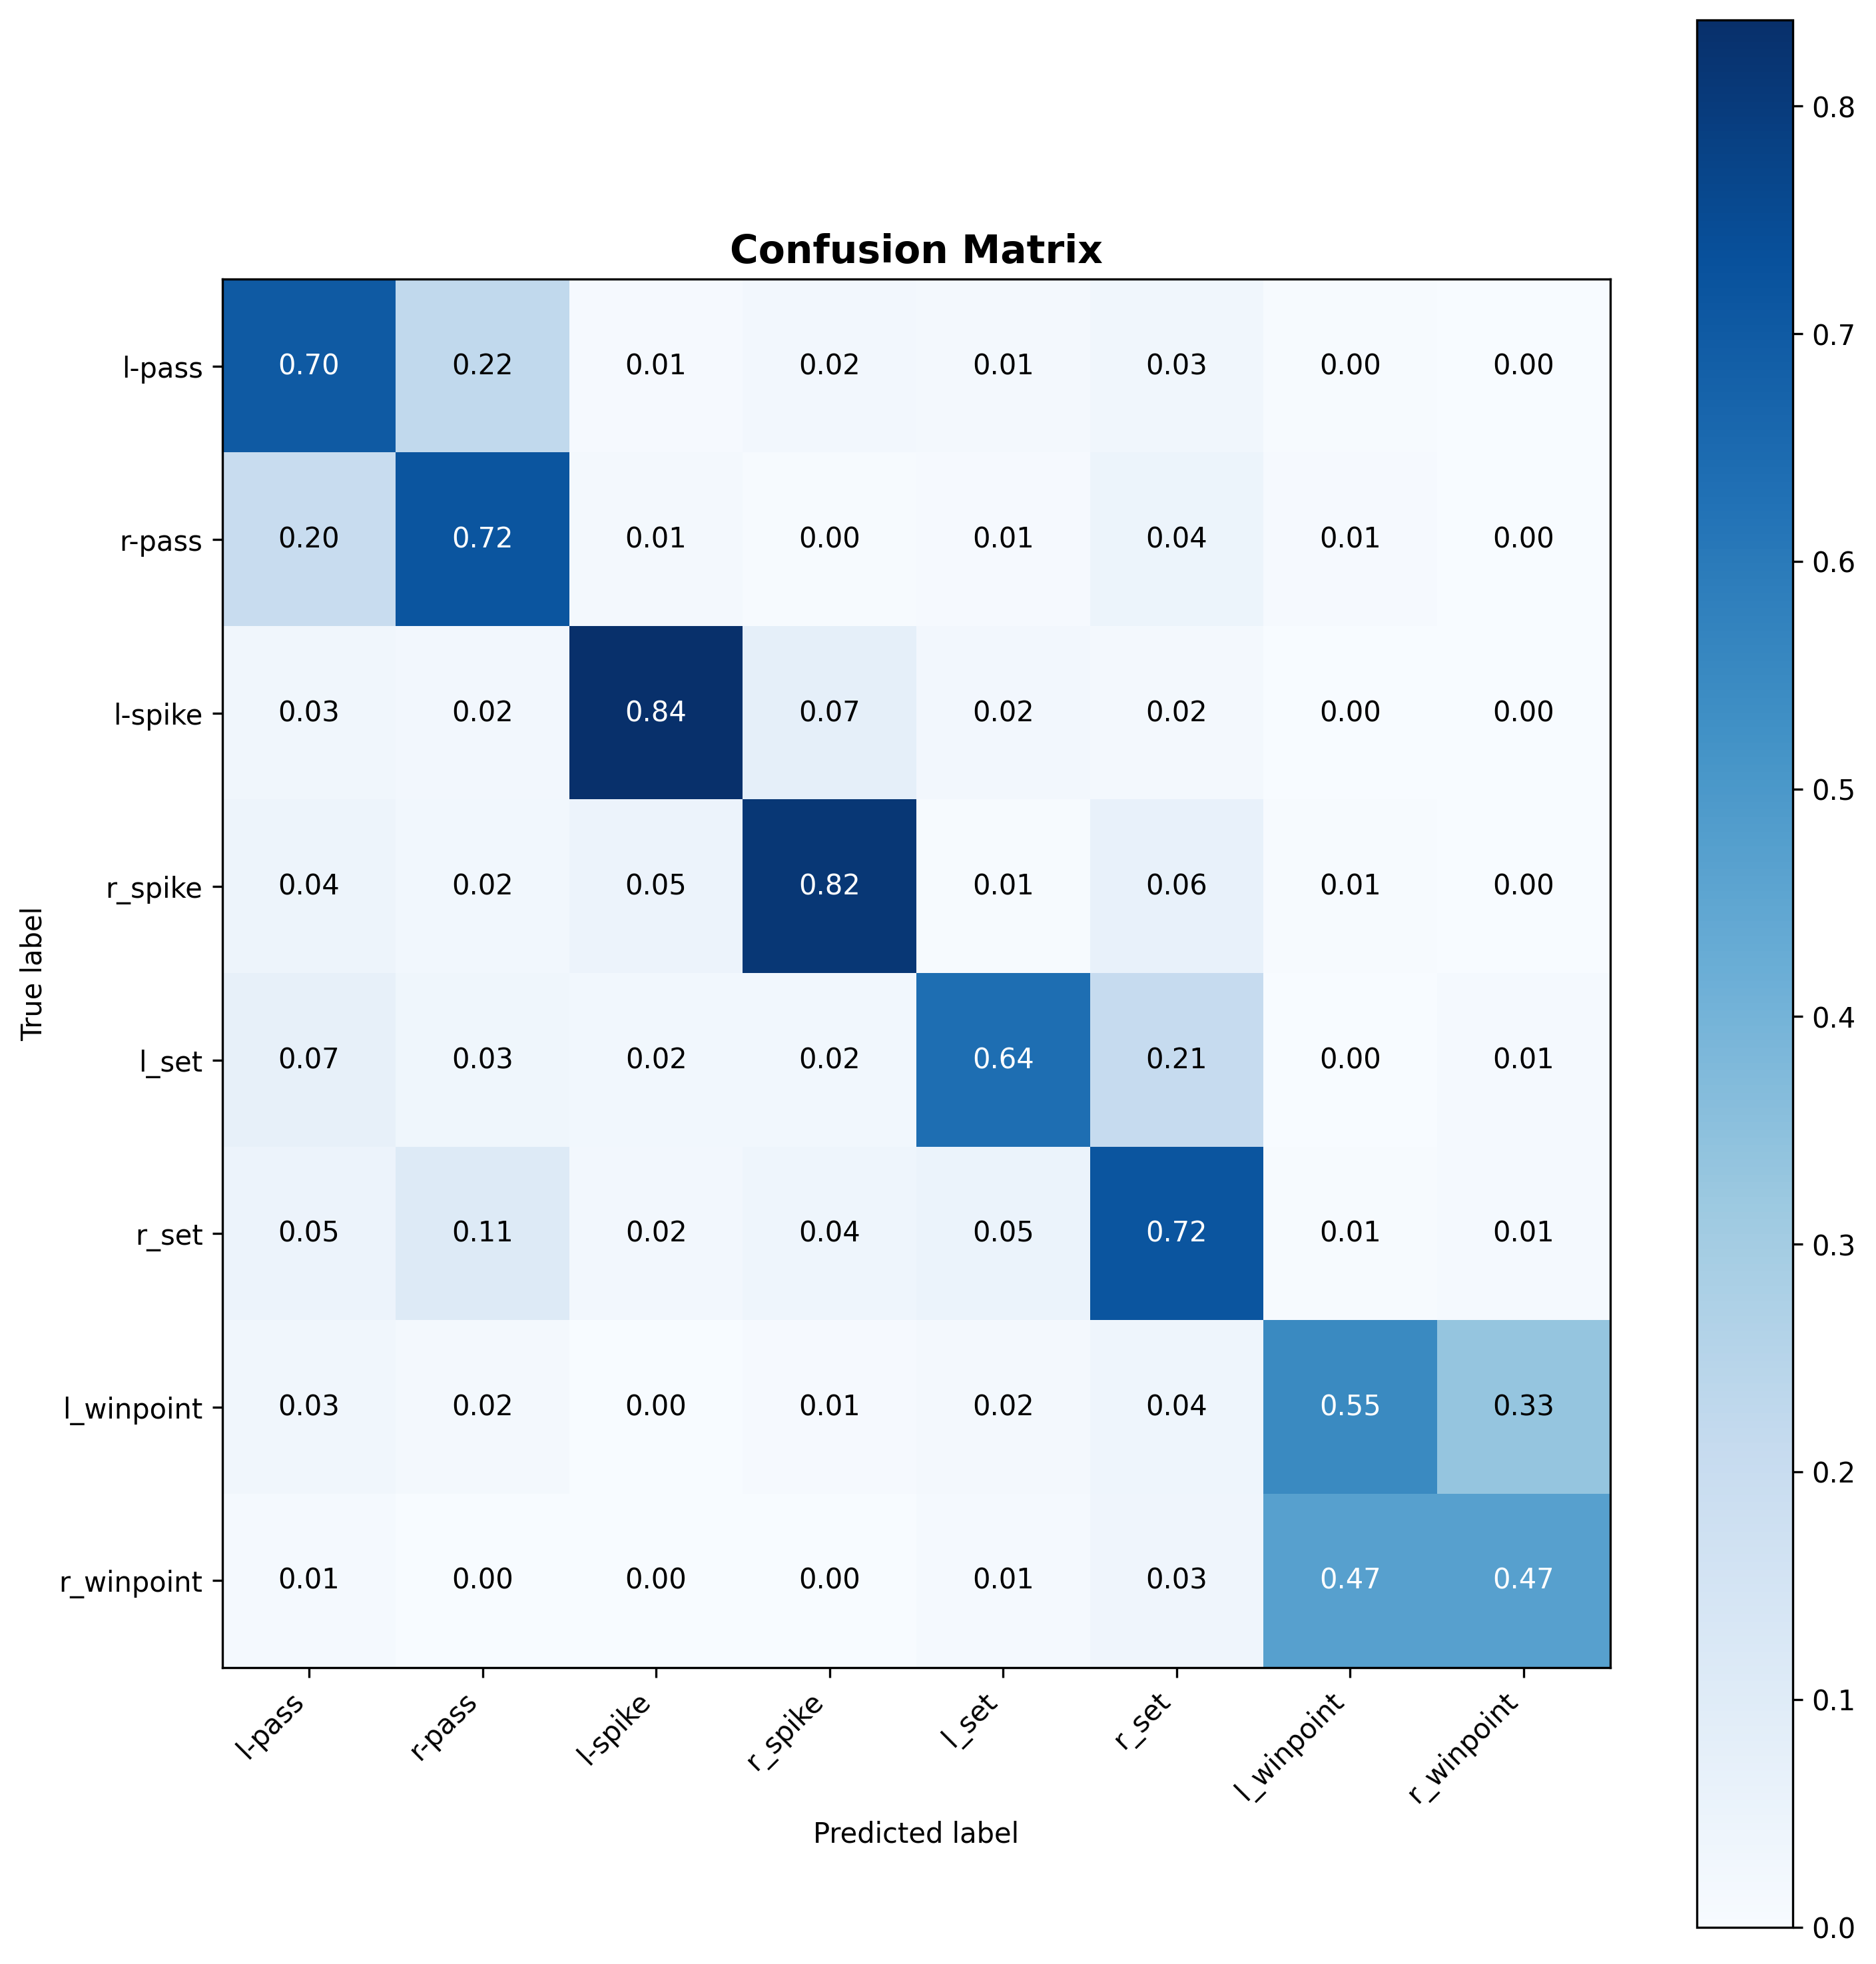
\includegraphics[width=0.95\linewidth]{figures/b6_confusion_matrix.png}
    \caption{Baseline 6 test confusion matrix. Winpoint recovers from B5's collapse (\texttt{r\_winpoint} recall $0.08 \to 0.47$), but left/right leakage --- winpoint, pass, and set --- is now the dominant error mode.}
    \label{fig:b6-confusion}
\end{figure}

\section{Baseline 7: Full Hierarchical Model}

B7 is the paper's two-stage hierarchical model with skip connections at both levels. A player-level \textbf{LSTM$_1$} runs over each player's 9-frame track; players are pooled per frame into a scene sequence that a scene-level \textbf{LSTM$_2$} consumes. Two skips are added on top of the paper: (1) \emph{player-level, feature-axis} --- each timestep's per-player vector is $[\text{LSTM}_1\text{ output} \,\|\, \text{Linear-projected backbone features}]$ (the paper's fc7 $\|$ hidden trick), keeping appearance beside the temporal summary while the time axis survives for LSTM$_2$; (2) \emph{scene-level, time-axis} --- B6's recipe of concatenating LSTM$_2$'s hidden states with a projection of the pooled scene sequence along time, then a global-kernel Conv1d fusion. Stage A pretrains LSTM$_1$ + projection on the 9 person actions (P$=$1 tracks); Stage B is two-phase (probe with the player model frozen, then joint fine-tune unfreezing LSTM$_1$), selecting on validation accuracy. Optimizer is AdamW.

\begin{table}[h]
    \centering
    \caption{Baseline 7 test-set metrics (run 3).}
    \label{tab:b7-metrics}
    \begin{tabular}{lc}
        \toprule
        \textbf{Metric} & \textbf{Value} \\
        \midrule
        Accuracy   & \textbf{73.75\%} \\
        Macro F1   & \textbf{0.701} \\
        Test Loss  & \textbf{0.89} \\
        \bottomrule
    \end{tabular}
\end{table}

B7 is the \textbf{strongest model without team-split pooling} (only B8 beats it): accuracy $+3.2$ points over B6 (73.8\% vs.\ 70.5\%), macro F1 0.701 vs.\ 0.686, and a lower test loss (0.89). The full hierarchy pays off --- an adapting player-level LSTM feeding a scene-level LSTM beats B6's single scene-level LSTM over pooled frames. The result hinges on the \textbf{two-phase Stage B}: with LSTM$_1$ frozen the probe plateaus at ${\sim}0.51$ validation accuracy, and unfreezing it for the joint fine-tune lifts validation accuracy to ${\sim}0.68$ ($+0.17$). This is the same lesson as B6 (pretrained temporal weights must adapt to the group task) and explains why B7's earlier \emph{frozen} single-phase run scored only 65.8\%, below B6 --- unfreezing turned that into $+7.9$ points. What B7 still does not fix is the left/right confusion: it pools all players side-blind, so winpoint/pass/set leak across sides. That is exactly B8's target.

\section{Baseline 8: Team-Split Pooling}

B8 makes a single architectural change to B7 --- the paper's group-style pooling. Instead of pooling all ${\sim}12$ players into one scene vector (side-blind), each team's players are pooled \emph{separately} and the two team vectors are concatenated, so the scene vector keeps \emph{which side did what} --- the signal every earlier baseline erases, and the direct fix for the dominant left/right confusion (winpoint, pass, set). Both of B7's skips are kept unchanged; only the scene vector doubles in width (LSTM$_2$ input becomes $4H_1$ for max/mean or $8H_1$ for concat). Team membership comes from the data loader in team mode (\texttt{with\_teams=True}), which emits a per-player \texttt{team\_ids} tensor (0/1 by court side, $-1$ for padding) derived once per clip from box center-$x$ ordering --- the paper's split, applied as a fixed per-track label so it coexists with the track-ID ordering the LSTMs require. Uneven or empty teams are handled by masking (a missing team pools to a zero vector).

\begin{table}[h]
    \centering
    \caption{Baseline 8 test-set metrics (run 1).}
    \label{tab:b8-metrics}
    \begin{tabular}{lc}
        \toprule
        \textbf{Metric} & \textbf{Value} \\
        \midrule
        Accuracy   & \textbf{85.64\%} \\
        Macro F1   & \textbf{0.855} \\
        Test Loss  & \textbf{0.51} \\
        \bottomrule
    \end{tabular}
\end{table}

B8 is the \textbf{best model in the project by a wide margin}: $+11.9$ accuracy and $+0.154$ macro F1 over B7 (85.6\% vs.\ 73.8\%), clearing the CVPR-2016 full model (81.9\%). The single change from B7 --- pooling each team separately --- is responsible, and its effect is visible exactly where predicted. As Fig.~\ref{fig:b8-confusion} shows, the \textbf{left/right confusion is fixed}: \texttt{r\_winpoint}, which collapsed to ${\sim}0.08$ recall in B5 and ${\sim}0.38$ in B7 (47\% predicted as \texttt{l\_winpoint}), now sits at \textbf{0.86} with 5\% cross-side leak, and \texttt{l\_winpoint} reaches 0.83; the l/r-pass swap (20--24\% in B6/B7) is gone (both 0.86--0.87); spike is near-perfect (0.93/0.90). What remains is \emph{within}-side confusion (e.g.\ \texttt{l\_set}$\to$\texttt{l\_spike} 12\%), not left/right --- the model now reliably knows which team acted. Team pooling is strong even without fine-tuning: the probe alone (LSTM$_1$ frozen) reached ${\sim}0.83$ validation accuracy, already above B7's fully-fine-tuned 0.68.

\begin{figure}[h]
    \centering
    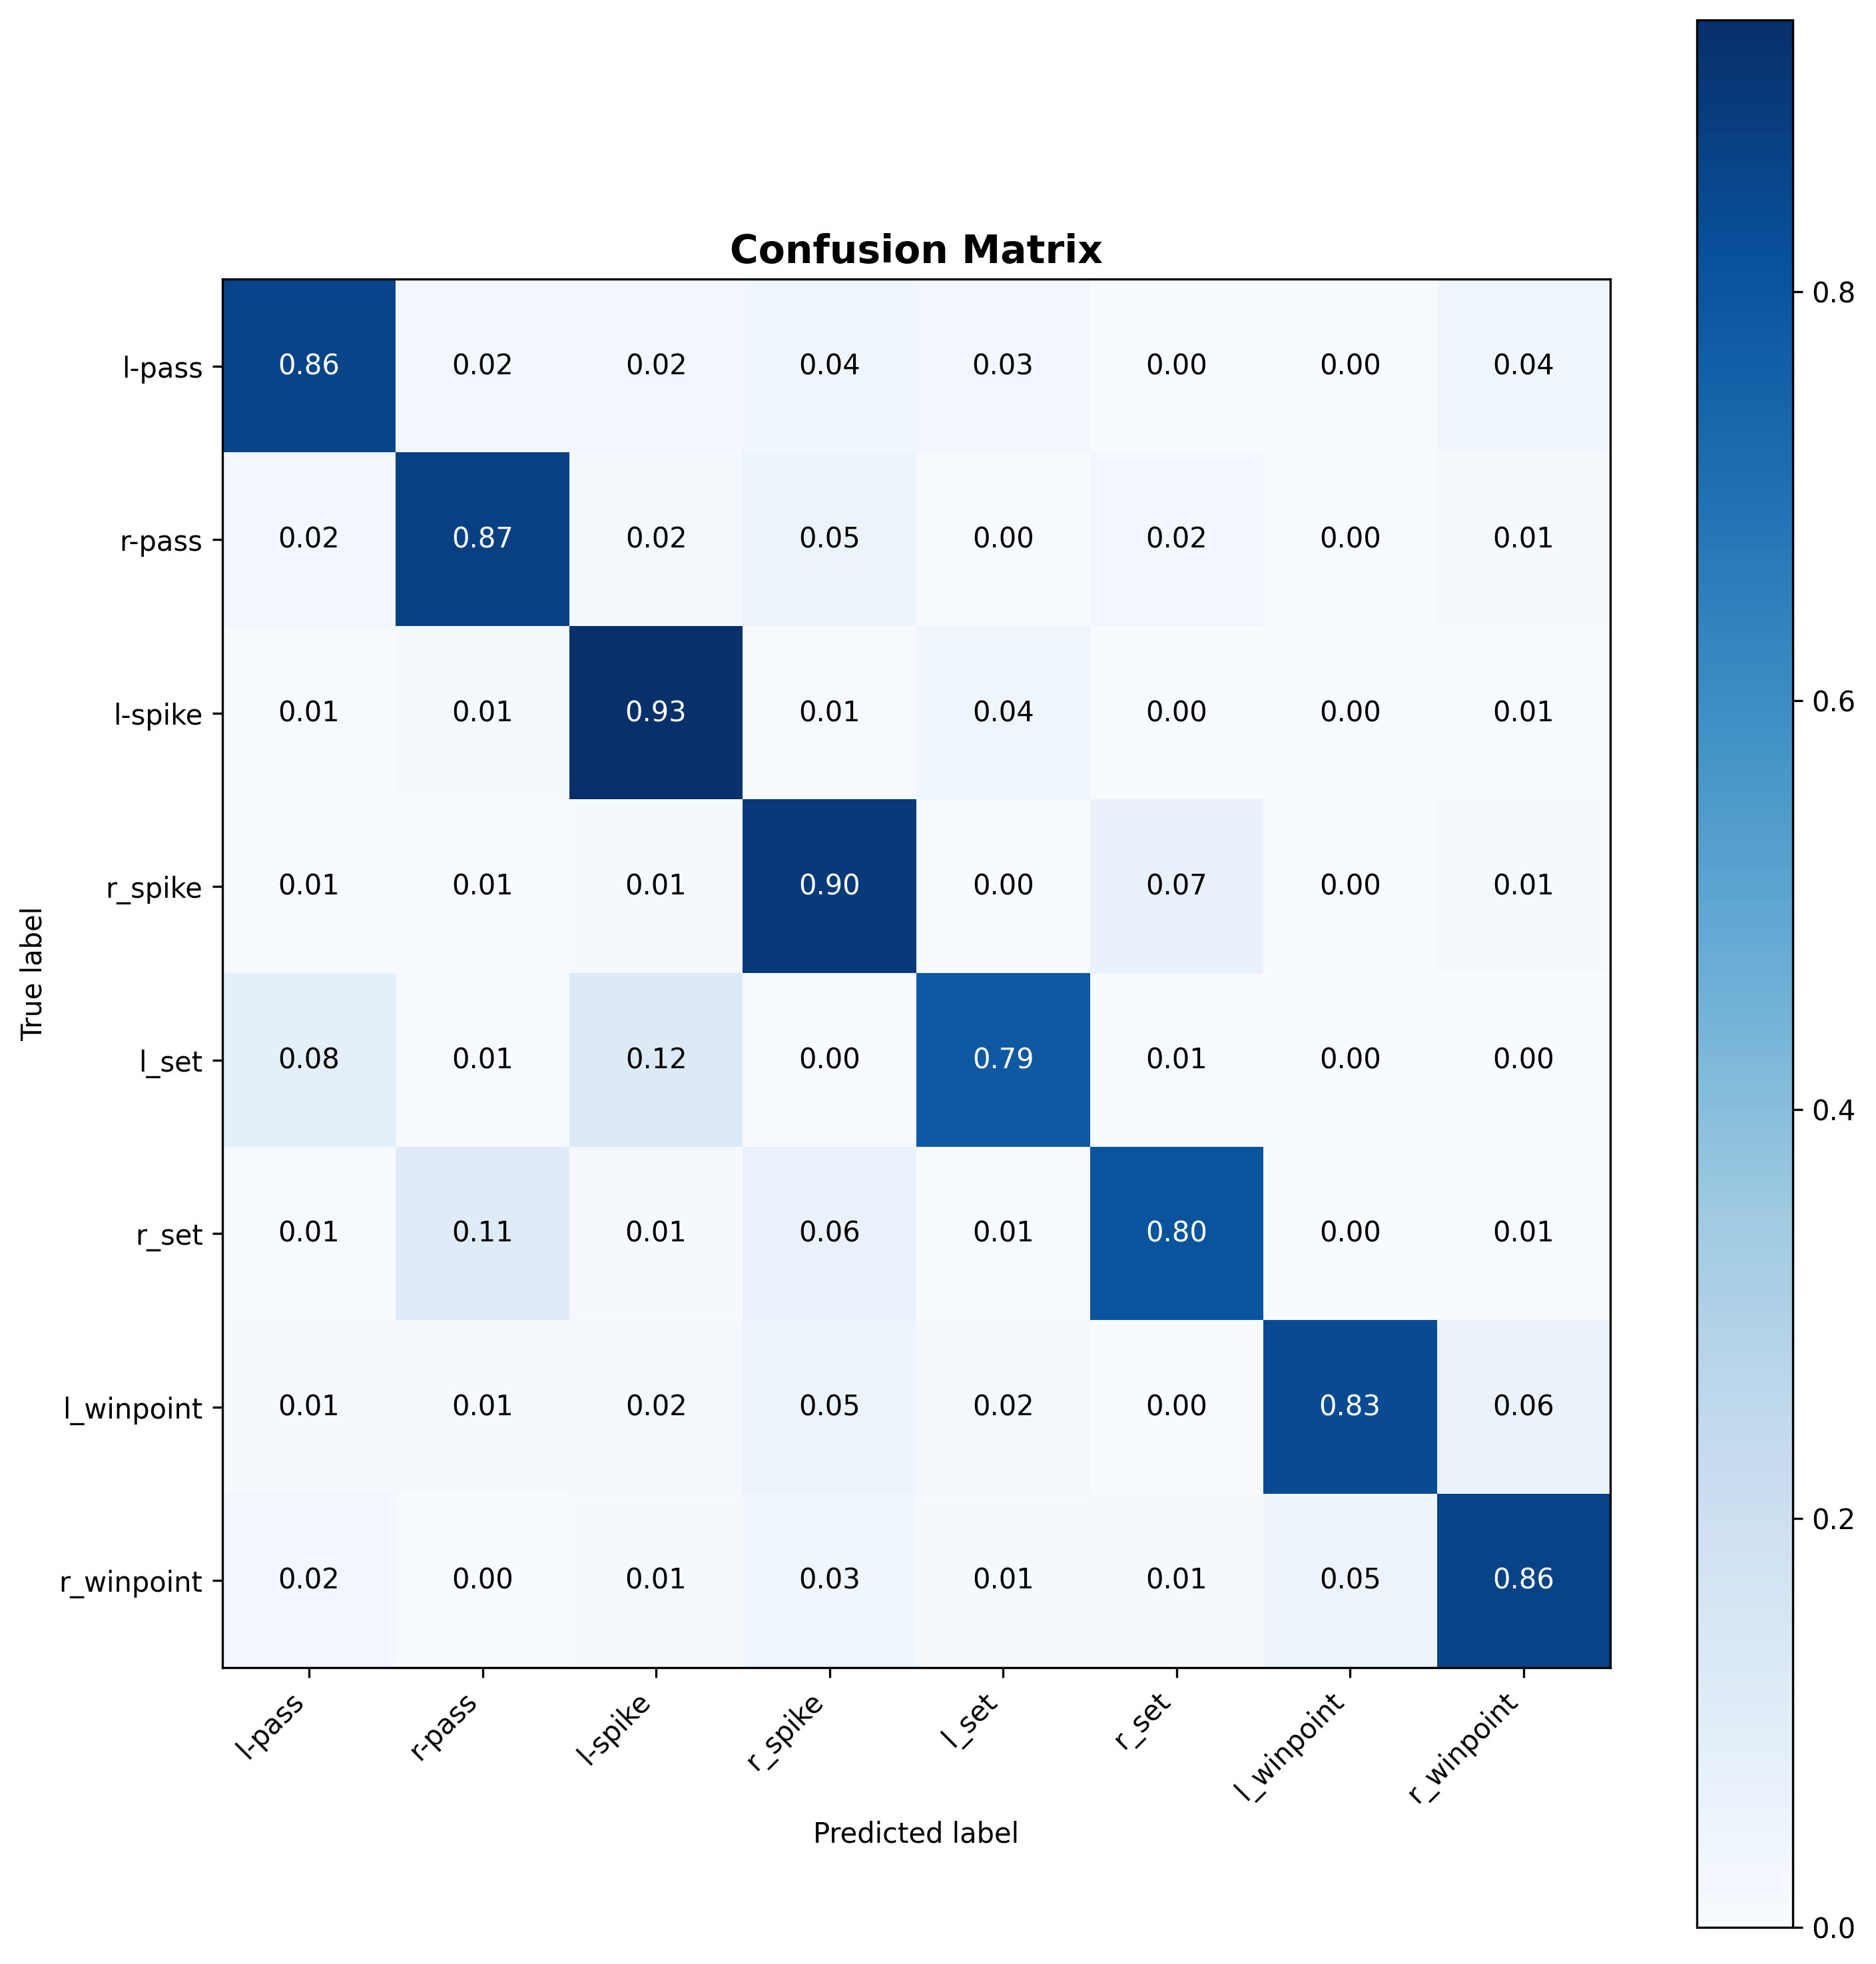
\includegraphics[width=0.95\linewidth]{figures/b8_confusion_matrix.png}
    \caption{Baseline 8 test confusion matrix. Team-split pooling eliminates the left/right leakage: winpoint recovers to 0.83/0.86 on the diagonal (from B7's ${\sim}0.38$), and pass/spike/set no longer swap sides. Remaining errors are within-side (e.g.\ set vs.\ spike).}
    \label{fig:b8-confusion}
\end{figure}

One caveat on the ablation: B8 used the \texttt{baseline3\_stage\_a\_run3} backbone while B7 used \texttt{run2} (person-action val acc 75.0\% vs.\ 70.4\%), so the $+11.9$ gain conflates team-split pooling with a slightly stronger backbone. The pooling is clearly dominant --- the paper's own team-pooling ablation is $+11.6$, and the probe-alone result isolates the effect --- but a perfectly clean comparison would re-run B7 on \texttt{run3}.

\section{Baseline 9: One Model, No Player Annotations}

Every baseline from B3 onward assumes the paper's premise: group activity is a function of what the individual players are doing, so the model needs boxes, tracks, person-action labels and a hierarchy to pool them. B9 tests that premise by discarding all of it. A single pretrained \textbf{YOLO26-x classifier} consumes the whole $224\times224$ frame and predicts one of the 8 group activities directly --- no detector head, no crops, no \texttt{team\_ids}, no LSTM, no staged schedule, and \emph{not one player annotation is read}. It is the ``throw a large pretrained model at it'' answer, included because it is the honest control for everything the ladder builds.

Two pieces of plumbing make it fit the project. \texttt{utils/yolo\_export.py} rewrites the same annotations into the ImageFolder layout Ultralytics requires, honouring the project's video split so the test set is the same 16 videos, and \emph{warps} frames to a square rather than symlinking them: Ultralytics' \texttt{Resize} + \texttt{CenterCrop} would discard 44\% of the court width, and with 8 classes in left/right pairs the court width \emph{is} the label. \texttt{utils/yolo\_probe.py} walks the scale ladder to find the largest architecture the GPU can train and ladders the batch size for it. Ultralytics owns the training loop, so B9 cannot use our \texttt{Trainer} to run --- but it still uses it as the \emph{log sink}: \texttt{Trainer.log\_epoch} and \texttt{Trainer.record\_test} are called from Ultralytics' own callbacks, so B9's scalars, per-epoch JSON and hyperparameter card come out in the same format as B1--B8, and \texttt{utils/evaluate.py} grew a YOLO path that emits the same four plots in the same class order.

\begin{table}[h]
    \centering
    \caption{Baseline 9 test-set metrics (run 3, the checkpoint on disk). Scored per frame over 13{,}370 test frames; B1--B8 are scored per clip over 1{,}337 clips.}
    \label{tab:b9-metrics}
    \begin{tabular}{lc}
        \toprule
        \textbf{Metric} & \textbf{Value} \\
        \midrule
        Accuracy        & \textbf{78.86\%} \\
        Macro F1        & \textbf{0.802} \\
        Top-5 accuracy  & 98.86\% \\
        Test Loss       & --- \\
        \bottomrule
    \end{tabular}
\end{table}

\textbf{B9 fails in the opposite direction from B1--B7.} The entire B5$\to$B8 storyline was left/right confusion: side-blind pooling drove \texttt{r\_winpoint} to 0.08 recall in B5 and 0.38 in B7, and team-split pooling was the fix. B9 does not have that problem. As Fig.~\ref{fig:b9-confusion} shows, its \emph{winpoints are its two best classes} (\texttt{l\_winpoint} 0.90, \texttt{r\_winpoint} 0.86, with 6--8\% cross-side leak), which is intuitive: a winpoint is a whole-scene state --- players scattered, celebrating --- and a full-frame model reads scene layout without needing to know who acted. What B9 loses is the fine-grained action distinction \emph{within} a side: the five largest off-diagonal cells are all same-side action swaps (\texttt{r\_set}$\to$\texttt{r-pass} 0.23, \texttt{l\_set}$\to$\texttt{l-pass} 0.17, \texttt{r-pass}$\to$\texttt{r\_set} 0.16, \texttt{r\_spike}$\to$\texttt{r\_set} 0.11, \texttt{l-pass}$\to$\texttt{l\_set} 0.11). Set and pass differ by one player's arm posture, and in a $224\times224$ full frame that player occupies roughly $17\times62$ pixels --- the evidence is not resolvable at that scale. Spike, which has a distinctive whole-body silhouette, survives at 0.87/0.82.

\begin{figure}[h]
    \centering
    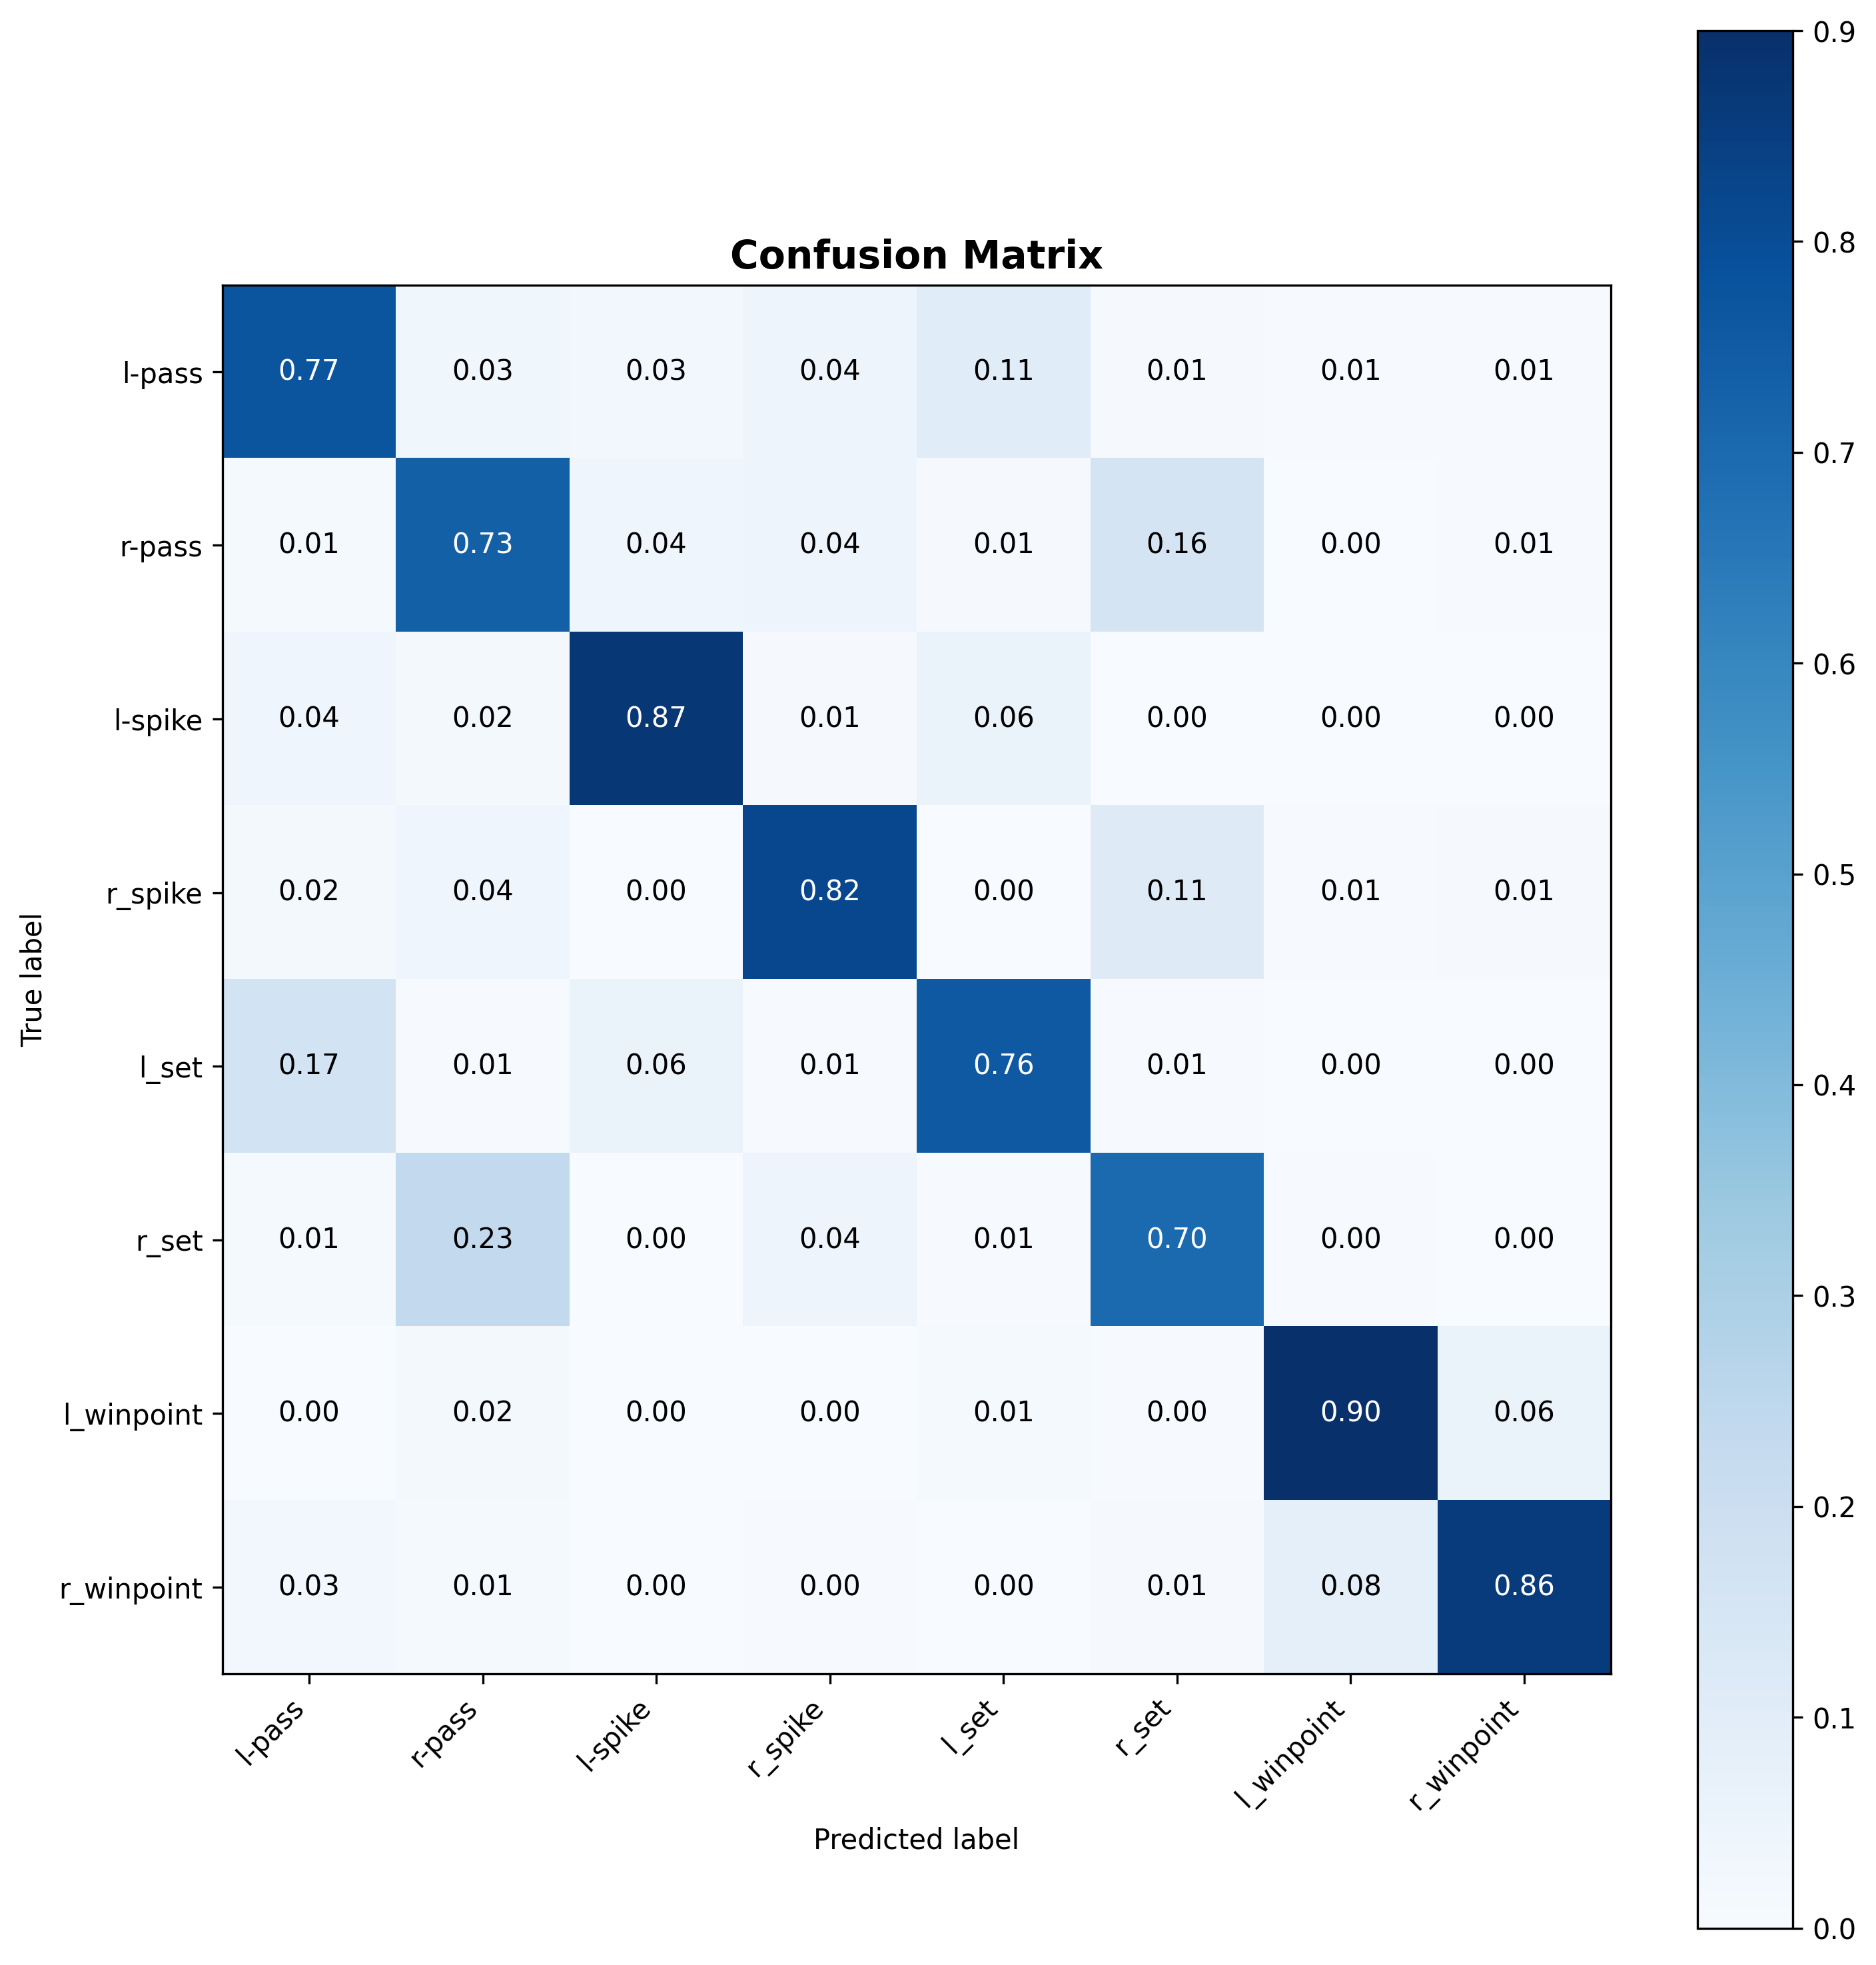
\includegraphics[width=0.95\linewidth]{figures/b9_confusion_matrix.png}
    \caption{Baseline 9 test confusion matrix. The left/right problem that dominated B5--B7 is absent --- winpoint is the strongest class (0.90/0.86) --- but set and pass swap \emph{within} a side (0.17--0.23), the distinction a $17\times62$-pixel player cannot support.}
    \label{fig:b9-confusion}
\end{figure}

This is precisely the trade the hierarchy makes explicit: \textbf{player crops buy resolution on the action; team-split pooling buys the side.} B9 gets the side for free from global scene layout and loses the action; B1--B7 got the action from crops and lost the side until B8 restored it. Quantitatively the hierarchy is worth roughly $+3$ to $+7$ accuracy points --- B8's 85.6\% against B9's 78.9\% for the plotted run, or against 83.2\% for B9's best run --- at the cost of the entire annotation stack (every box, every track, 9 person-action labels, a court-side assignment), a three-stage schedule and a pretrained person backbone, where B9 needs a directory of JPEGs in 8 folders. The ladder wins, and wins on macro F1 as well (0.855 vs.\ 0.846 at B9's best), but it is not the difference between working and not working.

Two caveats belong with these numbers. First, B9 \textbf{overfits hard}: by epoch 98 training loss is 0.0027 while validation loss has climbed to 1.93 from a minimum near 1.21. This is also the most likely explanation for an awkward result --- run 1, which used Ultralytics' \emph{default} random erasing (40\% of frames, up to a third of the frame blanked), scored 83.17\%/0.846, its best, while later runs with erasing dialled down to a player-sized box landed at 78.9--79.7\%. The aggressive occlusion was acting as the regularizer, even though it frequently erased the acting player outright. Second, run 1's weights were overwritten (Ultralytics reuses the run directory), so Table~\ref{tab:b9-metrics} and Fig.~\ref{fig:b9-confusion} report run 3, the checkpoint that still exists.

\section{Next Steps}

(i) \textbf{Clean the B7/B8 ablation} by re-running B7 on the \texttt{run3} backbone, so the $+11.9$ jump is attributed to team-split pooling alone. (ii) \textbf{Reduce overfitting} across all baselines --- stronger augmentation, higher dropout, and earlier stopping remain the levers (B8's fine-tune reaches ${\sim}97\%$ train accuracy against ${\sim}84\%$ validation). (iii) Beyond the ladder, the extension paper's graph/relational models are the natural next step for modeling inter-player structure explicitly rather than via pooling. (iv) \textbf{Two cheap wins on B9}: it is currently scored per frame while every other baseline is scored per clip, so a majority vote over each clip's frames would make the comparison like-for-like and should raise its number; and since its errors are dominated by a resolution limit (set vs.\ pass at $17\times62$ pixels), retraining at a larger \texttt{imgsz} probes the gap far more cheaply than the annotation pipeline does. (v) B9's own regularization needs a proper sweep rather than the accidental one described above --- the run that generalized best did so by erasing a third of the frame.

%----------------------------------------------------------

\end{document}
